\documentclass[sigconf]{webmedia}

\usepackage{lmodern}
\usepackage{graphicx}
\usepackage{float}

\AtBeginDocument{%
  \providecommand\BibTeX{{%
    \normalfont B\kern-0.5em{\scshape i\kern-0.25em b}\kern-0.8em\TeX}}}

\settopmatter{printacmref=false, printfolios=false}

\setevent{webmedia}
\proceedingsDetails[WebMedia'2026]{Proceedings of the Brazilian Symposium on Multimedia and the Web}{2026}{Lavras/MG, Brazil} 
\ISSN{2966-2753}

\begin{document}

\title{Análise Estrutural de Sentimentos sobre Entidades em Eventos utilizando Redes Bipartidas com Sinais}

\author{Pedro H. S. Oliveira}
\email{pedro.oliveira3@ufv.br}
\affiliation{%
  \institution{Universidade Federal de Viçosa (UFV) - Viçosa, MG, Brasil}
}

\renewcommand{\shortauthors}{Oliveira, P. H. S.}

\begin{abstract}
Este artigo final descreve uma metodologia estruturada para análise de sentimentos em eventos utilizando o modelo de Redes Bipartidas com Sinais. Com dados oriundos de logs de avaliações voluntárias extraídas da plataforma myMobiConf, exploramos como as redes unipartidas sinalizadas projetadas revelam bolhas de opiniões de participantes, polarização sobre aspectos e heterogeneidade de interação que métricas percentuais globais (como o Net Sentiment Score) ignoram ou enviesam, oferecendo um diagnóstico topológico profundo de eventos e experiências sociais.
\end{abstract}

\keywords{Redes Bipartidas Sinalizadas, Análise de Sentimentos, Gephi, Eventos Acadêmicos, myMobiConf}

\maketitle

\section{Introdução e Motivação}

O gerenciamento de eventos acadêmicos e corporativos modernos tem se apoiado em soluções móveis e ubíquas como a plataforma myMobiConf \cite{oliveira}. O myMobiConf é um sistema ciente de contexto e distribuído, desenvolvido para auxiliar na organização de eventos e conferências acadêmicas, empresariais e tecnológicas, buscando proporcionar uma experiência mais interativa e eficiente \cite{peixoto2026}. A plataforma é composta por três módulos principais: um aplicativo móvel para os participantes, um dashboard web destinado aos organizadores, e um backend responsável pelo processamento e integração dos dados. Durante o evento, o sistema coleta feedbacks e avaliações dos participantes, os quais enviam opiniões textuais voluntárias sobre diversos aspectos, tais como palestrantes, sessões, internet Wi-Fi ou coffee break. Essa dinâmica gera um volume massivo de dados qualitativos. No estágio pós-evento, são realizadas análises que resultam em uma série de relatórios, como relatórios de comentários narrativos, análises de questionários e diagnóstico das programações. Embora o sistema preserve a privacidade por meio da descaracterização dos dados, é possível correlacionar as diferentes manifestações enviadas pelo mesmo usuário anônimo ao longo do evento através de seu identificador de sessão.

Tradicionalmente, a análise de feedback de eventos na indústria baseia-se fortemente em métricas agregadas univariadas. O Net Sentiment Score (NSS) \cite{reichheld, reyes}, por exemplo, condensa a saúde do evento em uma fórmula baseada puramente em volume:

\begin{equation}
\text{NSS} = \frac{\text{Positivos} - \text{Negativos}}{\text{Total de Comentários}} \times 100
\end{equation}

Apesar de sua utilidade para gestão, pesquisadores alertam que abordagens focadas apenas no número final escondem a complexidade das opiniões humanas \cite{liu, taboada}. O NSS e médias parecidas resumem excessivamente as informações, destruindo a rede de interações que se forma naturalmente. O ato de somar ou fazer a média das avaliações facilita que usuários fora do padrão manipulem as notas gerais \cite{akoglu2013, kumar2018}. Por isso, analisar o evento como uma rede tornou-se essencial para descobrir quem são os usuários confiáveis e qual é a verdadeira qualidade dos serviços.

Pela visão da Teoria de Redes Complexas \cite{barabasi, newman}, um evento é um ambiente muito conectado, onde as opiniões criam um mapa direto (um grafo bipartido) entre as pessoas e os detalhes da conferência. Ao ignorar esse formato, as métricas tradicionais não respondem a perguntas básicas sobre o feedback:

\begin{enumerate}
    \item Heterogeneidade de Usuários: A participação das pessoas varia muito \cite{easley}. Usando algoritmos de rede \cite{kumar2018}, é possível saber se uma nota baixa foi dada por muitas pessoas comuns, indicando uma falha geral, ou se foi culpa de um único usuário que reclamou dezenas de vezes.
    \item Formação de Bolhas de Opinião: As avaliações não acontecem de forma isolada, e a literatura de polarização mostra que as pessoas tendem a se dividir em grupos com opiniões fortes \cite{alsinet2023, candellone2024}. Modelos baseados apenas em porcentagens são cegos para essas bolhas e não conseguem agrupar usuários que pensam de forma parecida.
    \item Correlação de Aspectos: É preciso separar as opiniões por assunto \cite{wu}. Em redes desse tipo, onde não existem triângulos, usamos ciclos de quatro pontos (borboletas sinalizadas) para aplicar teorias de equilíbrio \cite{derr2019}. Isso nos ajuda a investigar se uma reclamação sobre o Wi-Fi, por exemplo, acaba contaminando a nota da organização geral do evento.
\end{enumerate}

Diante dessa perda drástica de informações, argumentamos que depender apenas de porcentagens não é suficiente para entender o comportamento das pessoas nos eventos. 

Para resolver isso, este trabalho levanta a hipótese de que as opiniões em um evento formam naturalmente uma rede complexa. Manter o formato original dessa rede preserva detalhes fundamentais que seriam apagados ao usar apenas médias numéricas \cite{huang2021, gu2024}. Assim, defendemos que analisar o formato (topologia) dessa rede revela informações essenciais, como a verdadeira variação de engajamento, as bolhas de opinião e a relação entre os itens avaliados. Esses fenômenos simplesmente desaparecem quando limitamos a análise às métricas estatísticas tradicionais.

O projeto é orientado por cinco Questões de Pesquisa centrais aplicadas ao conjunto de dados de cada evento:
\begin{itemize}
    \item QP1 (Concentração e Polarização): Quais entidades de um evento concentram a maior carga de sentimentos positivos, negativos ou neutros, e qual é o saldo estrutural de sentimento de cada uma?
    \item QP2 (Heterogeneidade dos Usuários): Como se distribui o volume de feedback por usuário? A atividade de feedback é pulverizada de forma homogênea ou dominada por poucos super-usuários engajados?
    \item QP3 (Bolhas de Opinião Compartilhada): É possível agrupar os usuários em comunidades baseando-se unicamente na similaridade de suas percepções sobre as mesmas entidades (projeção unipartida de usuários)?
    \item QP4 (Correlação Estrutural de Aspectos): Quais entidades ou serviços do evento tendem a ser avaliados conjuntamente pelos mesmos participantes, revelando padrões de dependência de experiência (projeção unipartida de entidades)?
    \item QP5 (Sentimento Geral do Evento): Como o sentimento geral e agregado do evento (NSS Global tradicional de mercado) se comporta e se compara com as métricas estruturais do grafo?
\end{itemize}

\section{Trabalhos Relacionados}

A modelagem de sentimentos por meio de grafos tem se expandido rapidamente na literatura, superando a análise tradicional de textos isolados. Os trabalhos que fundamentam essa pesquisa dividem-se em três grandes frentes focadas em confiabilidade, agrupamento social e processamento estrutural profundo.

\subsection{Confiabilidade e Detecção de Fraudes em Avaliações}
Na área de comércio eletrônico e plataformas de avaliações, pesquisadores comprovaram que calcular médias gerais de notas é um método falho. Ferramentas como o algoritmo FRAUDEAGLE \cite{akoglu2013} e o sistema REV2 \cite{kumar2018} utilizam redes bipartidas que conectam pessoas aos produtos que elas avaliam. O objetivo dessas ferramentas é detectar manipulações de opinião, isolando usuários excessivamente críticos ou fraudulentos e descobrindo a verdadeira qualidade das entidades avaliadas. O nosso trabalho aplica exatamente essa lógica investigativa aos eventos: em vez de apenas somar feedbacks, mapeamos a rede para entender se uma reclamação no myMobiConf reflete uma falha real na organização ou apenas a postura de um usuário atípico.

\subsection{Polarização e Bolhas em Redes Bipartidas}
É comum ouvirmos falar sobre "bolhas" na internet, onde pessoas que pensam igual conversam apenas entre si. A maioria das pesquisas estuda esse fenômeno observando quem fala com quem. Porém, a ciência de redes descobriu que a polarização também acontece quando as pessoas não conversam entre si, mas interagem com os mesmos tópicos ou produtos \cite{alsinet2023}. Mesmo sem diálogo direto, o público se divide naturalmente em grupos fechados que avaliam as coisas exatamente da mesma forma \cite{candellone2024}. Essa descoberta é o que embasa a nossa Questão de Pesquisa 3: nós buscamos encontrar essas bolhas de opinião dentro do evento, agrupando os participantes que concordam entre si sobre a qualidade das palestras e da organização, independentemente de se conhecerem.

\subsection{Preservação Estrutural e Correlação de Aspectos}
Pesquisas em redes neurais (como SBGNN \cite{huang2021} e ELISE \cite{gu2024}) provam que transformar redes bipartidas em métricas simples destrói padrões de comportamento latentes. Alinhado a isso, nosso trabalho preserva a rede original do evento para não perder nenhuma nuance das avaliações. Além disso, aplicamos o conceito de "borboletas sinalizadas" (ciclos de quatro pontos para redes bipartidas) introduzido por Derr et al. \cite{derr2019}. Essa base técnica é o que nos permite investigar a correlação de aspectos (Questão de Pesquisa 4): ou seja, medir matematicamente se a insatisfação do participante com um serviço específico (como o Wi-Fi) contamina estruturalmente as notas que ele dá para os outros setores do evento.

\subsection{A Ponte com Redes Sociais Fictícias}
O artigo de Nonaka e Perry (2026) \cite{nonaka}, "Evaluating LLM Story Generation through Large-scale Network Analysis of Social Structures", serve como principal inspiração metodológica. Eles aplicaram a teoria das redes para analisar histórias geradas por inteligência artificial, mapeando as interações amigáveis ou hostis entre personagens fictícios. Enquanto o trabalho deles foca em grafos unipartidos na ficção, este projeto adapta a modelagem e traz as métricas sinalizadas para as Redes Bipartidas do mundo físico. Dessa forma, mapeamos a realidade das conferências acadêmicas, conectando o comportamento humano verdadeiro à estrutura dos serviços do myMobiConf.

\section{Metodologia}

A modelagem baseia-se na extração de entidades e sentimentos dos logs de comentários salvos, seguindo um fluxo metodológico estruturado em cinco pilares fundamentais, ilustrados na Figura \ref{fig:workflow} e descritos nas seções a seguir.

\begin{figure}[h]
  \centering
  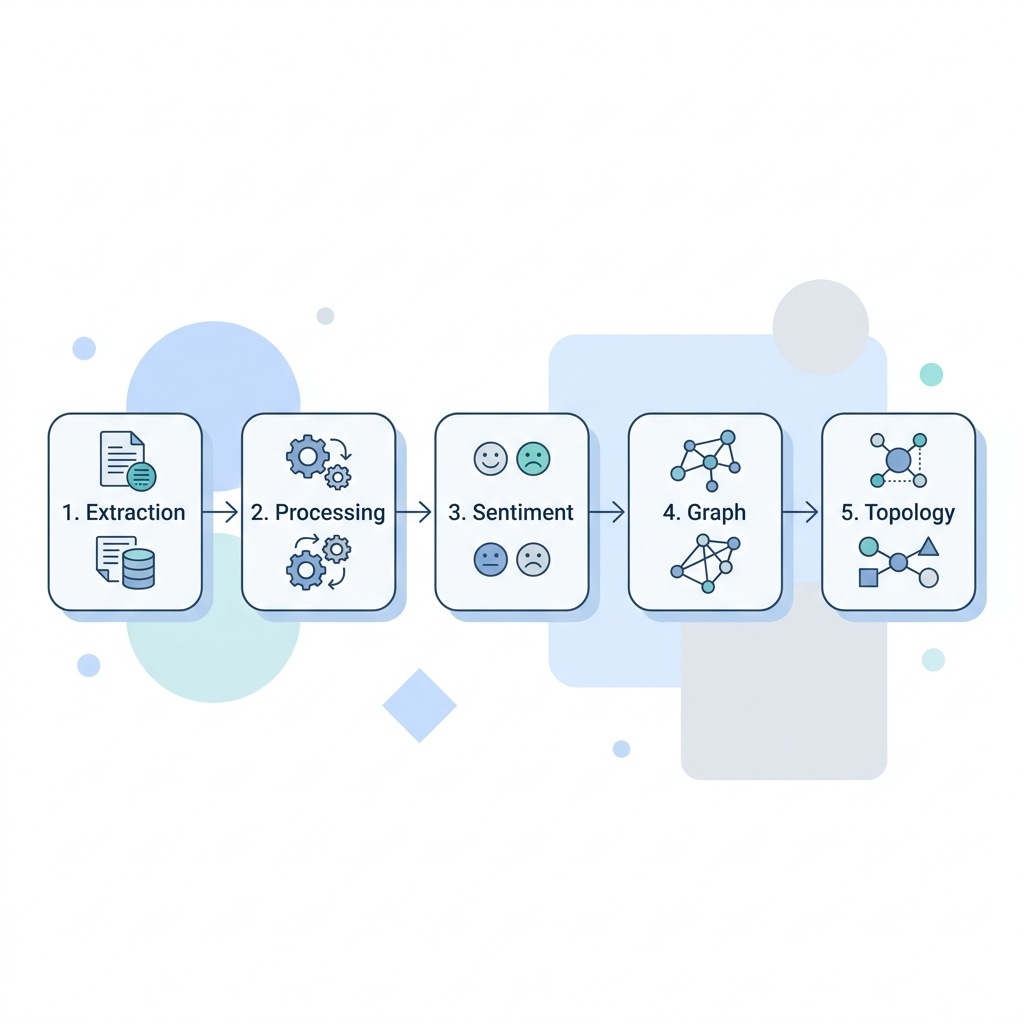
\includegraphics[width=\linewidth]{workflow.png}
  \caption{Workflow metodológico estrutural do projeto.}
  \label{fig:workflow}
\end{figure}

\subsection{Extração dos Dados}
Para validar a metodologia, extraímos a base de logs brutos da plataforma myMobiConf \cite{oliveira}. Os comentários coletados foram rigorosamente anonimizados por meio de \textit{hashes} para preservar a privacidade dos participantes. Selecionamos seis eventos com dinâmicas variadas, cobrindo desde conferências massivas até workshops menores, visando garantir que o modelo de redes seja robusto diante de diferentes perfis de engajamento, conforme apresentado na Tabela \ref{tab:volume}. Analisar os eventos de forma independente é vital para não misturar os contextos das entidades avaliadas.

\subsection{Processamento dos Dados}
O processamento ocorre em duas frentes complementares: o tratamento inicial focado em padronização (Limpeza) e a segmentação semântica (\textit{Sentence Splitting}). 

\subsubsection{Tratamento de Dados Iniciais}
A primeira fase do processamento tem como objetivo mitigar a severa despadronização característica de mídias sociais. Aplicamos a conversão de todos os caracteres para letras minúsculas (\textit{lowercasing}) e a remoção sistemática de URLs e artefatos de código HTML, como quebras de linha sujas. Emojis, que frequentemente carregam a principal carga semântica do comentário, são tratados para que os algoritmos léxicos consigam interpretá-los na etapa seguinte. Além disso, removemos \textit{logs} duplicados submetidos pelo mesmo participante em um curto intervalo de tempo; essa deduplicação é de suma importância para evitar que o envio massivo de reclamações (\textit{flood}) infle artificialmente o peso final da aresta no grafo.

\subsubsection{Segmentação Semântica (Sentence Splitting)}
O segundo passo resolve a alta densidade de comentários compostos. É rotineiro que participantes redijam longos parágrafos relatando diversas experiências simultâneas. O \textit{Sentence Splitting} utiliza o \textit{pipeline} do spaCy para detectar fronteiras sintáticas, quebrando os blocos de texto em orações semânticas independentes. A divisão ocorre por meio de pontuações fortes (ponto final, exclamação) e também identificando conjunções coordenativas adversativas e aditivas, a exemplo de "e", "mas" e "porém". 

Esta quebra sintática possui uma justificativa matemática essencial para a integridade da rede: se um participante escreve "A palestra foi ótima, mas o Wi-Fi estava lento", a avaliação tradicional de sentenças longas resultaria em uma polaridade neutra e entidades embaralhadas. Ao separar as sentenças, o sistema consegue criar duas arestas distintas no grafo direcionado: uma aresta altamente positiva apontando para "Palestra" e outra aresta negativa apontando para "Wi-Fi". Isso mapeia o sentimento do usuário com precisão. Como demonstrado empiricamente na Tabela \ref{tab:volume}, a etapa de \textit{splitting} expande sensivelmente o volume de instâncias disponíveis para modelagem.

\begin{table}[h]
\centering
\caption{Evolução do volume de dados da Extração ao Processamento.}
\label{tab:volume}
\resizebox{\linewidth}{!}{
\begin{tabular}{lrrr}
\hline
\textbf{Evento} & \textbf{Extração Bruta} & \textbf{Limpeza} & \textbf{Pós-Processamento (Split)} \\
\hline
Evento 1 & 1.857 & 1.796 & 2.050 \\
Evento 2 & 1.206 & 1.198 & 1.601 \\
Evento 3 & 642 & 599 & 651 \\
Evento 4 & 75 & 74 & 117 \\
Evento 5 & 24 & 24 & 29 \\
Evento 6 & 12 & 12 & 21 \\
\hline
\end{tabular}
}
\end{table}

\subsection{Análise de Sentimento e Extração de Aspectos}
A decisão arquitetural para a identificação das entidades (aspectos) diverge significativamente da literatura recente. Enquanto trabalhos como o de Nonaka e Perry \cite{nonaka} dependem de grandes modelos de linguagem (LLMs) para mapear redes sociais, essa abordagem apresenta severas barreiras de custo computacional e latência quando aplicada a um sistema em produção como o myMobiConf, que processa milhares de logs informais continuamente. Por outro lado, o uso tradicional de dicionários estáticos falha diante da variação vocabular, de gírias e de erros ortográficos naturais no contexto de eventos.

Por isso, a abordagem mais recomendada e adotada neste trabalho é uma modelagem \textit{bottom-up} combinando Processamento de Linguagem Natural clássico com representações vetoriais densas. Primeiramente, a biblioteca spaCy \cite{spacy} realiza o \textit{POS-Tagging} para extrair substantivos que são candidatos a entidades. Na sequência, em vez de depender de uma validação de dicionário fechado, os candidatos são projetados em embeddings de 384 dimensões via \textit{Sentence-Transformers} \cite{reimers}. O diferencial central desta escolha técnica reside na robustez da capacidade semântica latente: um algoritmo não-supervisionado de Agrupamento Aglomerativo funde palavras que compartilham a mesma vizinhança vetorial - a exemplo de "app", "aplicativo", "sistema" e até falhas ortográficas como "aplcativo" -, baseando-se puramente na distância do cosseno. O termo mais frequente torna-se o nó canônico da rede bipartida. Essa abordagem constrói agrupamentos perfeitamente orgânicos das entidades mais comentadas no evento, descartando a necessidade de \textit{prompts} não determinísticos ou do alto custo de chamadas de API externas em tempo real, garantindo máxima escalabilidade e controle local.

Simultaneamente, o cálculo da polaridade das arestas (o peso $w$ do sentimento associado à entidade) no intervalo $[-1, 1]$ é realizado utilizando o LeIA (Léxico para Inferência Adaptada), focado na língua portuguesa e derivado metodologicamente do algoritmo VADER \cite{vader}. A escolha do LeIA como o método mais recomendado para o contexto do myMobiConf baseia-se em dois grandes pilares: eficiência computacional e adaptação a microtextos. Diferente de modelos de \textit{Deep Learning} focados na língua portuguesa (como o BERTimbau), que exigem pesados recursos de hardware (GPUs) e grandes volumes de dados rotulados para \textit{fine-tuning}, o LeIA oferece uma abordagem \textit{zero-shot} baseada em regras léxicas, operando com baixíssima latência e sem necessidade de treinamento prévio na nuvem.

Além de ser leve, o LeIA foi desenvolvido especificamente para textos de mídias sociais e mensagens curtas, o que espelha exatamente a realidade de um evento, onde os comentários costumam ser redigidos às pressas nos smartphones, carregando forte informalidade, sarcasmo e intensificadores gramaticais. Diferente de analisadores léxicos tradicionais (baseados em \textit{Bag-of-Words}) que falham ao tratar apenas a soma de palavras positivas e negativas de forma isolada, o LeIA implementa heurísticas léxico-sintáticas avançadas. Ele ajusta a polaridade captando pontuação de ênfase ("ótimo!!!") e palavras em caixa alta ("EXCELENTE"), modula a intensidade através de advérbios de grau ("muito ruim" altera o peso final mais do que apenas "ruim"), e inverte matematicamente o sentimento ao encontrar partículas de negação (ex: "o café não estava bom"). Essa sensibilidade estrutural faz do LeIA a ferramenta ideal para capturar o real engajamento emocional dos participantes sem a sobrecarga de redes neurais profundas.

\subsection{Montagem do Grafo Bipartido Sinalizado}
Os dados extraídos na fase anterior fundamentam a construção da estrutura principal do estudo: o Grafo Bipartido Sinalizado e Direcionado, denotado formalmente por $G = (U, E, A, w)$. 

Nesta estrutura formal:
\begin{itemize}
    \item $U = \{u_1, u_2, \dots, u_n\}$ representa o conjunto de nós de usuários anonimizados participantes do evento.
    \item $E = \{e_1, e_2, \dots, e_m\}$ representa o conjunto de nós de entidades (aspectos canônicos comentados, como "Palestra", "Wi-Fi" ou "Organização").
    \item $A \subseteq U \times E$ é o conjunto de arestas direcionadas $(u, e)$ que existem se e somente se o usuário $u$ comentou sobre a entidade $e$.
    \item $w: A \rightarrow [-1, 1]$ é a função de peso da aresta, onde $w(u,e)$ indica a polaridade e a intensidade do sentimento de $u$ sobre $e$, extraída pelo léxico LeIA. Valores próximos a $1$ indicam extremo elogio, próximos a $-1$ indicam extrema frustração, e $0$ indica neutralidade.
\end{itemize}

Esta modelagem, ilustrada visualmente na Figura \ref{fig:bipartite}, é de suma importância porque preserva o mapeamento topológico exato de "quem avaliou o quê" e "com qual emoção".

\begin{figure}[h]
  \centering
  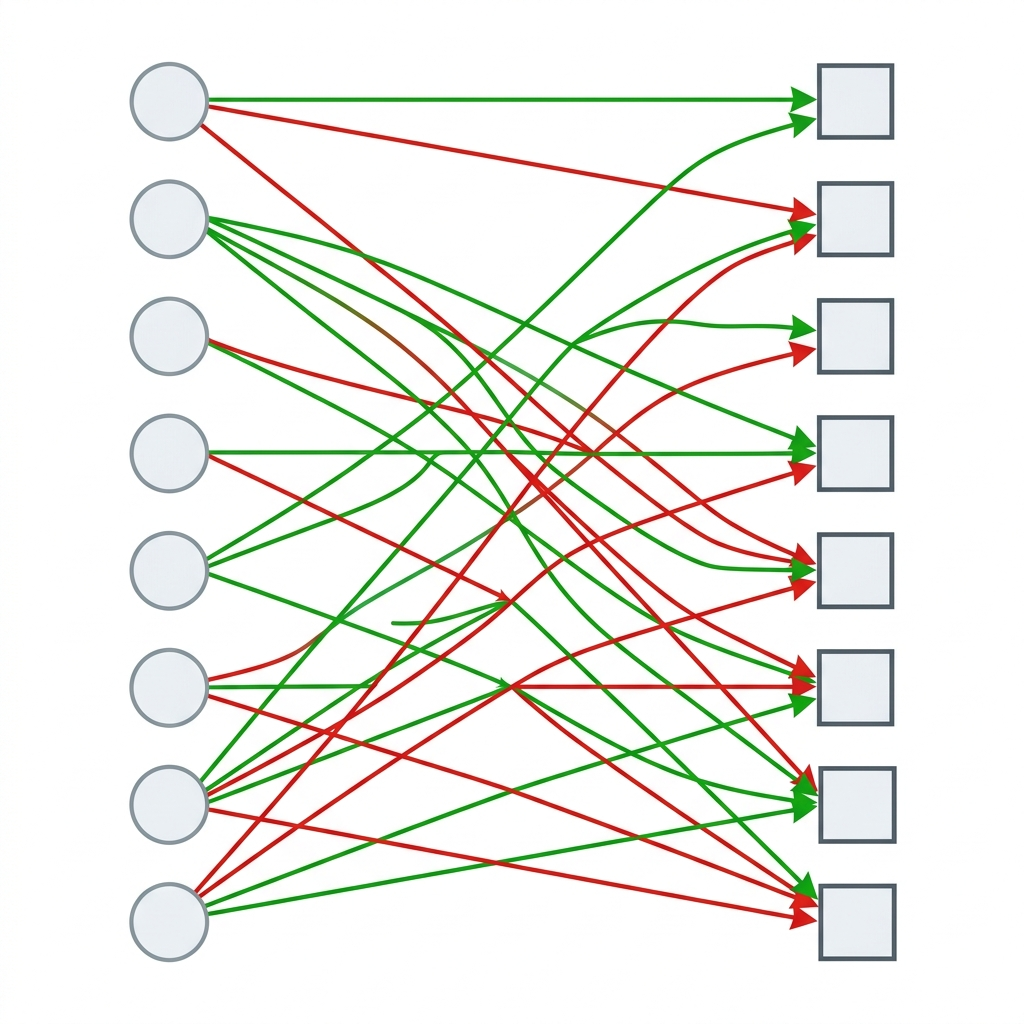
\includegraphics[width=0.8\linewidth]{bipartite_graph.png}
  \caption{Representação visual do Grafo Bipartido Sinalizado: Usuários (círculos) avaliando Entidades (quadrados) com sentimentos variados em verde e vermelho.}
  \label{fig:bipartite}
\end{figure}

\subsection{Análise Topológica e Subgrafos Projetados}
Embora o grafo bipartido $G$ mapeie a realidade crua das avaliações, a literatura de redes complexas demonstra que a correlação de comportamentos é melhor investigada através de projeções matemáticas unipartidas \cite{newman}. Ao projetar a rede, "dobramos" a estrutura bipartida para investigar relacionamentos indiretos. Neste trabalho, deduzimos duas projeções principais para a análise:

1. Projeção de Usuários ($G_{user}$): Neste subgrafo, os nós são exclusivamente os participantes ($U$). Uma aresta $(u_i, u_j)$ é criada se ambos comentaram sobre pelo menos uma entidade em comum. O peso $W_{u_i, u_j}$ dessa nova aresta é formalmente definido pelo produto escalar dos sentimentos que ambos emitiram para as entidades compartilhadas:
\begin{equation}
W_{u_i, u_j} = \sum_{e \in E} w(u_i, e) \cdot w(u_j, e)
\end{equation}
Em suma, esta fórmula reflete a \textit{concordância de opiniões}: se $u_i$ e $u_j$ deram notas com a mesma polaridade (ambos amaram ou ambos odiaram) para a mesma entidade $e$, o produto matemático dos sinais resulta em um incremento positivo para o peso da aresta. Se eles discordaram (sinais opostos), o peso da aresta sofre um decréscimo. Dessa forma, a função primária de $G_{user}$ torna-se mapear a homofilia \cite{easley}. Através da aplicação de algoritmos de detecção de comunidades, como o algoritmo de Louvain \cite{blondel}, segmentamos a rede para encontrar bolhas topológicas de opinião. Isso nos permite descobrir grupos isolados de usuários que viveram a mesma experiência no evento (ex: uma bolha focada estritamente no networking vs. uma bolha que concentrou reclamações de infraestrutura).

2. Projeção de Entidades ($G_{entity}$): Neste subgrafo, os nós são exclusivamente as entidades do evento ($E$). Uma aresta $(e_i, e_j)$ é formada se ambas foram comentadas em conjunto pelos mesmos usuários simultaneamente. O peso $W_{e_i, e_j}$ desta aresta é definido matematicamente por:
\begin{equation}
W_{e_i, e_j} = \sum_{u \in U} w(u, e_i) \cdot w(u, e_j)
\end{equation}
Em suma, a fórmula revela se duas áreas do evento estão sistemicamente interligadas na mente dos participantes. Se os usuários tendem a avaliar $e_i$ e $e_j$ com a mesma emoção (ex: reclamando de ambas juntas), o produto dos sentimentos é positivo, conferindo às entidades uma forte aresta de co-ocorrência sentimental. Consequentemente, a função de $G_{entity}$ é investigar a correlação estrutural dos aspectos. Em eventos, a experiência do participante é sistêmica: a frustração com o credenciamento inicial ($e_i$) pode contaminar a percepção subjetiva da primeira palestra ($e_j$). Mapeando essas ligações e calculando métricas de centralidade (como o Grau Ponderado), identificamos quais serviços são os pilares críticos de influência que sustentam - ou derrubam - o humor geral do evento.

Ao final deste pipeline, os grafos bipartidos e suas projeções unipartidas são exportados no formato GEXF \cite{bastian} para visualização espacial profunda em softwares especializados, encerrando o fluxo metodológico e fundamentando as respostas às Questões de Pesquisa.

\begin{figure}[h]
  \centering
  \begin{minipage}{0.48\linewidth}
    \centering
    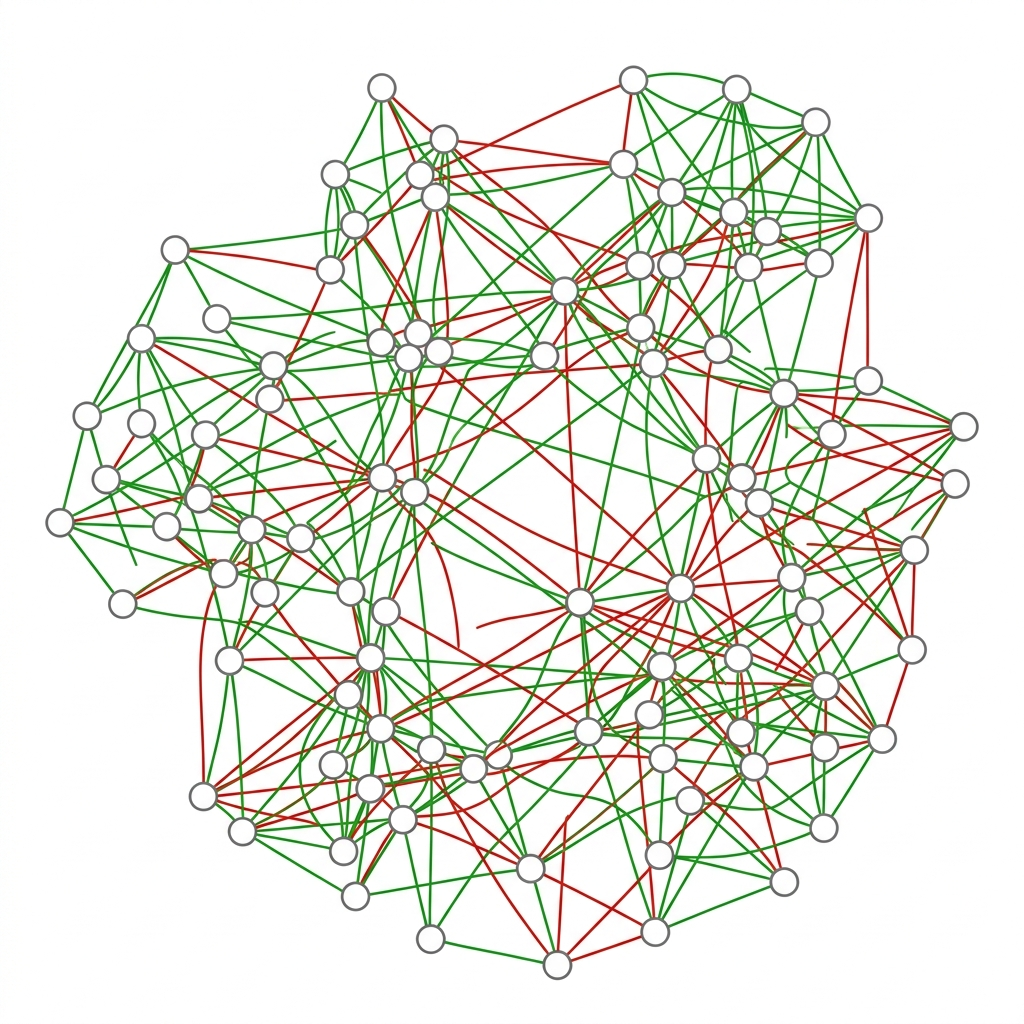
\includegraphics[width=\linewidth]{subgraph_user.png}
    \caption{Projeção $G_{user}$: as arestas indicam concordância ou discordância.}
    \label{fig:subgraph_user}
  \end{minipage}\hfill
  \begin{minipage}{0.48\linewidth}
    \centering
    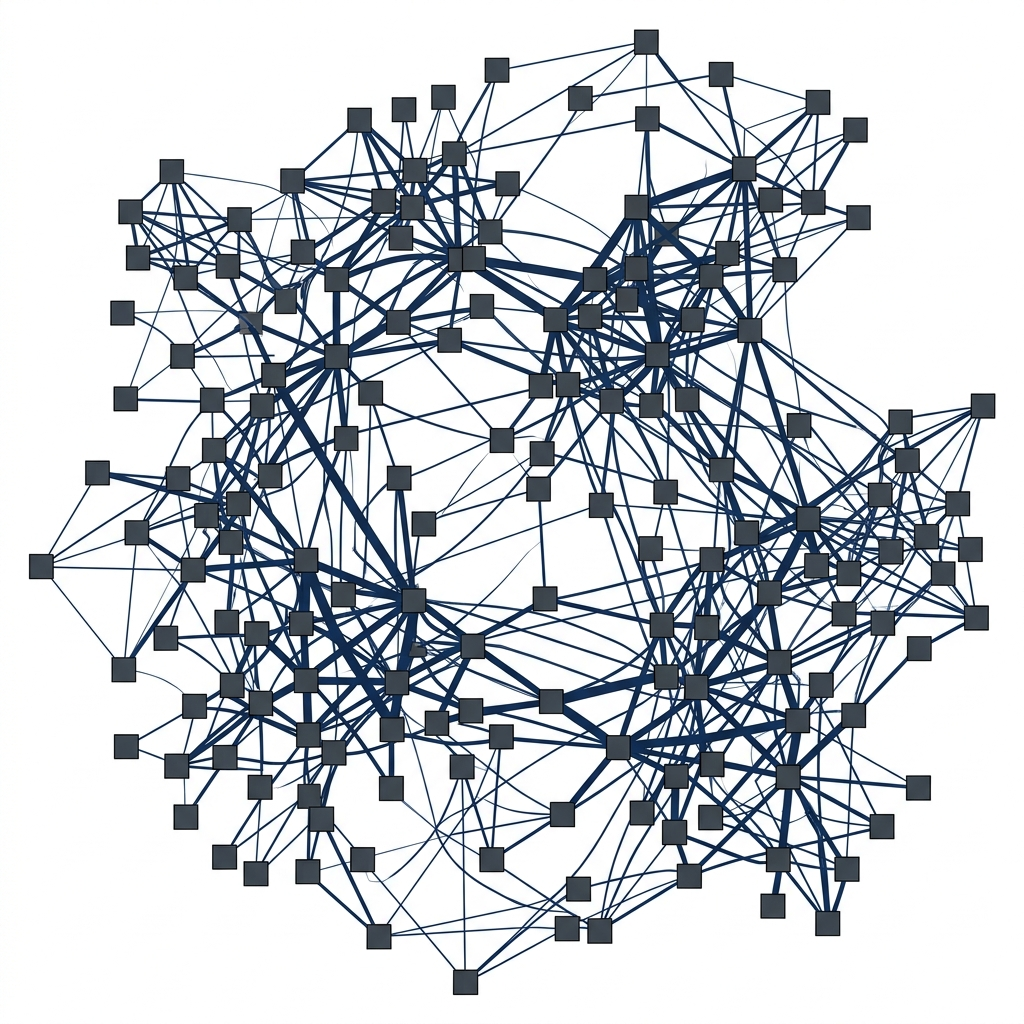
\includegraphics[width=\linewidth]{subgraph_entity.png}
    \caption{Projeção $G_{entity}$: as arestas mapeiam a correlação estrutural.}
    \label{fig:subgraph_entity}
  \end{minipage}
\end{figure}

\section{Resultados e Discussão}

\subsection{Critérios de Análise das Redes Geradas}

Antes de iniciar a análise dos eventos, definimos o panorama geral dos três grafos exportados e os critérios topológicos que fundamentam a avaliação empírica:

\begin{itemize}
    \item Rede Bipartida Sinalizada: Modela a relação Usuário $\rightarrow$ Aspecto.
    \item Projeção de Usuários ($G_{user}$): Conecta participantes por homofilia avaliativa \cite{easley}.
    \item Projeção de Entidades ($G_{entity}$): Conecta serviços do evento por correlação de experiência.
\end{itemize}

Com base nestes grafos, as cinco Questões de Pesquisa (QPs) são respondidas utilizando as seguintes métricas de redes complexas:
\begin{itemize}
    \item QP1 (Concentração e Polarização): Analisada prioritariamente via Grau de Entrada e Grau Ponderado para identificar grandes \textit{hubs}, utilizando o Net Sentiment Score (NSS) da entidade apenas como validador secundário de polaridade.
    \item QP2 (Heterogeneidade dos Usuários): Analisada via distribuição de \textit{out-degree}, buscando identificar padrões de cauda longa (\textit{scale-free}) \cite{barabasi}.
    \item QP3 (Bolhas de Opinião): Extração de comunidades na projeção de usuários ($G_{user}$) usando o algoritmo Louvain \cite{blondel}.
    \item QP4 (Correlação de Aspectos): Detecção de módulos semânticos de serviços codependentes ($G_{entity}$).
    \item QP5 (Intensidade da Rede vs. Saldo Comercial): Análise do peso médio das arestas (sentimento real da rede), utilizando o NSS global tradicional apenas como \textit{baseline} comparativo.
\end{itemize}

\subsection{Estudo de Caso: Evento 1 (Engajamento Muito Alto)}

\begin{figure}[H]
  \centering
  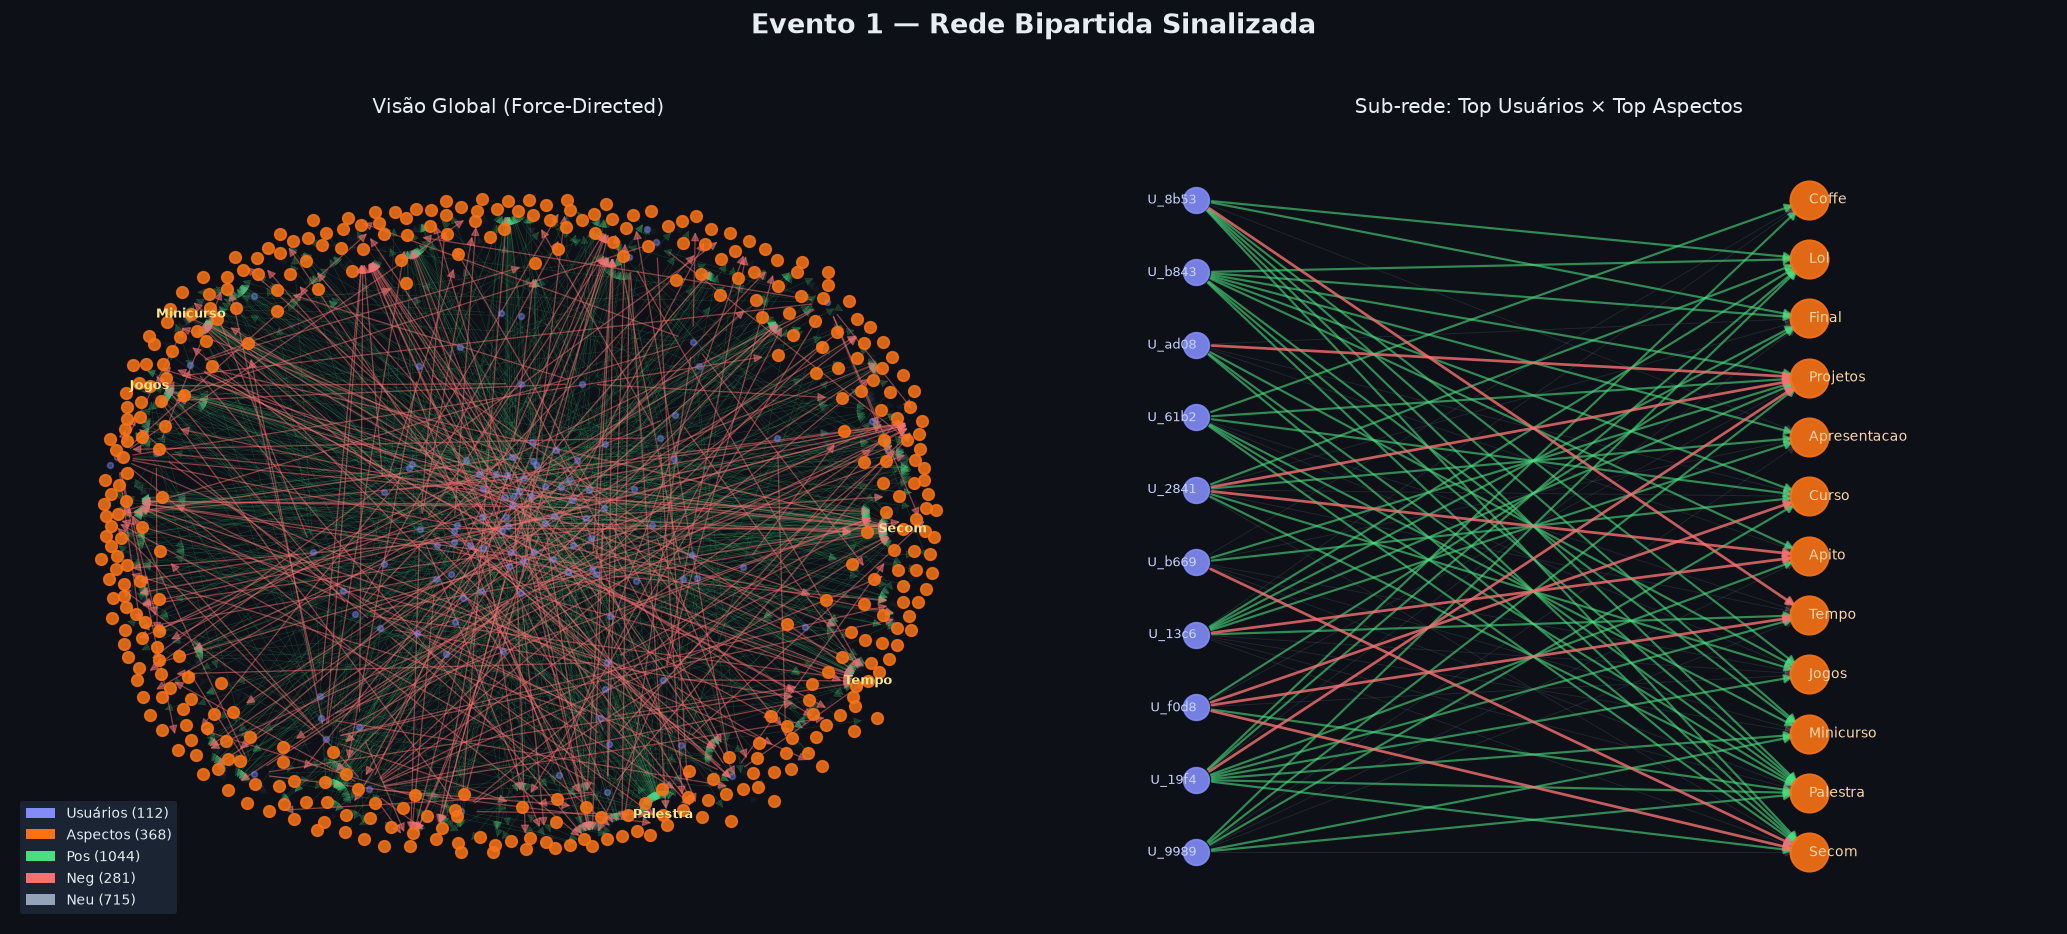
\includegraphics[width=\linewidth]{../resultados/redes/network_secom_xiii.png}
  \caption{Rede Bipartida Sinalizada - Evento 1.}
  \label{fig:evt1}
\end{figure}

Esta rede apresentou alta dispersão semântica. A estrutura foi modelada com 480 nós (112 usuários, 368 aspectos) e 2.040 arestas sinalizadas (1.044 positivas, 281 negativas, 715 neutras). A proporção de 3,28 aspectos por usuário indica grande riqueza de detalhes avaliados.

QP1 - Concentração e Polarização: Os grandes \textit{hubs} topológicos foram Secom (grau = 104), Palestra (grau = 83) e Minicurso (grau = 58). Esses nós absorveram as emoções positivas. Críticas foram focadas em aspectos menores e isolados (ex: Preconceitos, grau = 1). A métrica de NSS confirmou a polaridade esperada para esses hubs.

QP2 - Heterogeneidade: A participação foi surpreendentemente homogênea. Apenas 1,8\% dos usuários emitiram 1 feedback; 78,6\% enviaram 10 ou mais. Isso denota um público uniformemente ativo.

QP3 e QP4 - Bolhas e Correlação: Detectou-se apenas 8 comunidades de usuários, demonstrando altíssima coesão estrutural e consenso da audiência. O vocabulário rico gerou 60 comunidades de entidades, com forte separação topológica entre infraestrutura operacional e conteúdo.

QP5 - Intensidade e Sentimento Global: O Sentimento Médio (peso das arestas) foi de +0,179. Revelou-se um engajamento ativo, mas acompanhado de forte posicionamento crítico (13,8\% de arestas negativas). Como linha de base comparativa, o NSS da rede situou-se em 37,40\%.

\subsection{Estudo de Caso: Evento 2 (Engajamento Muito Alto)}

\begin{figure}[H]
  \centering
  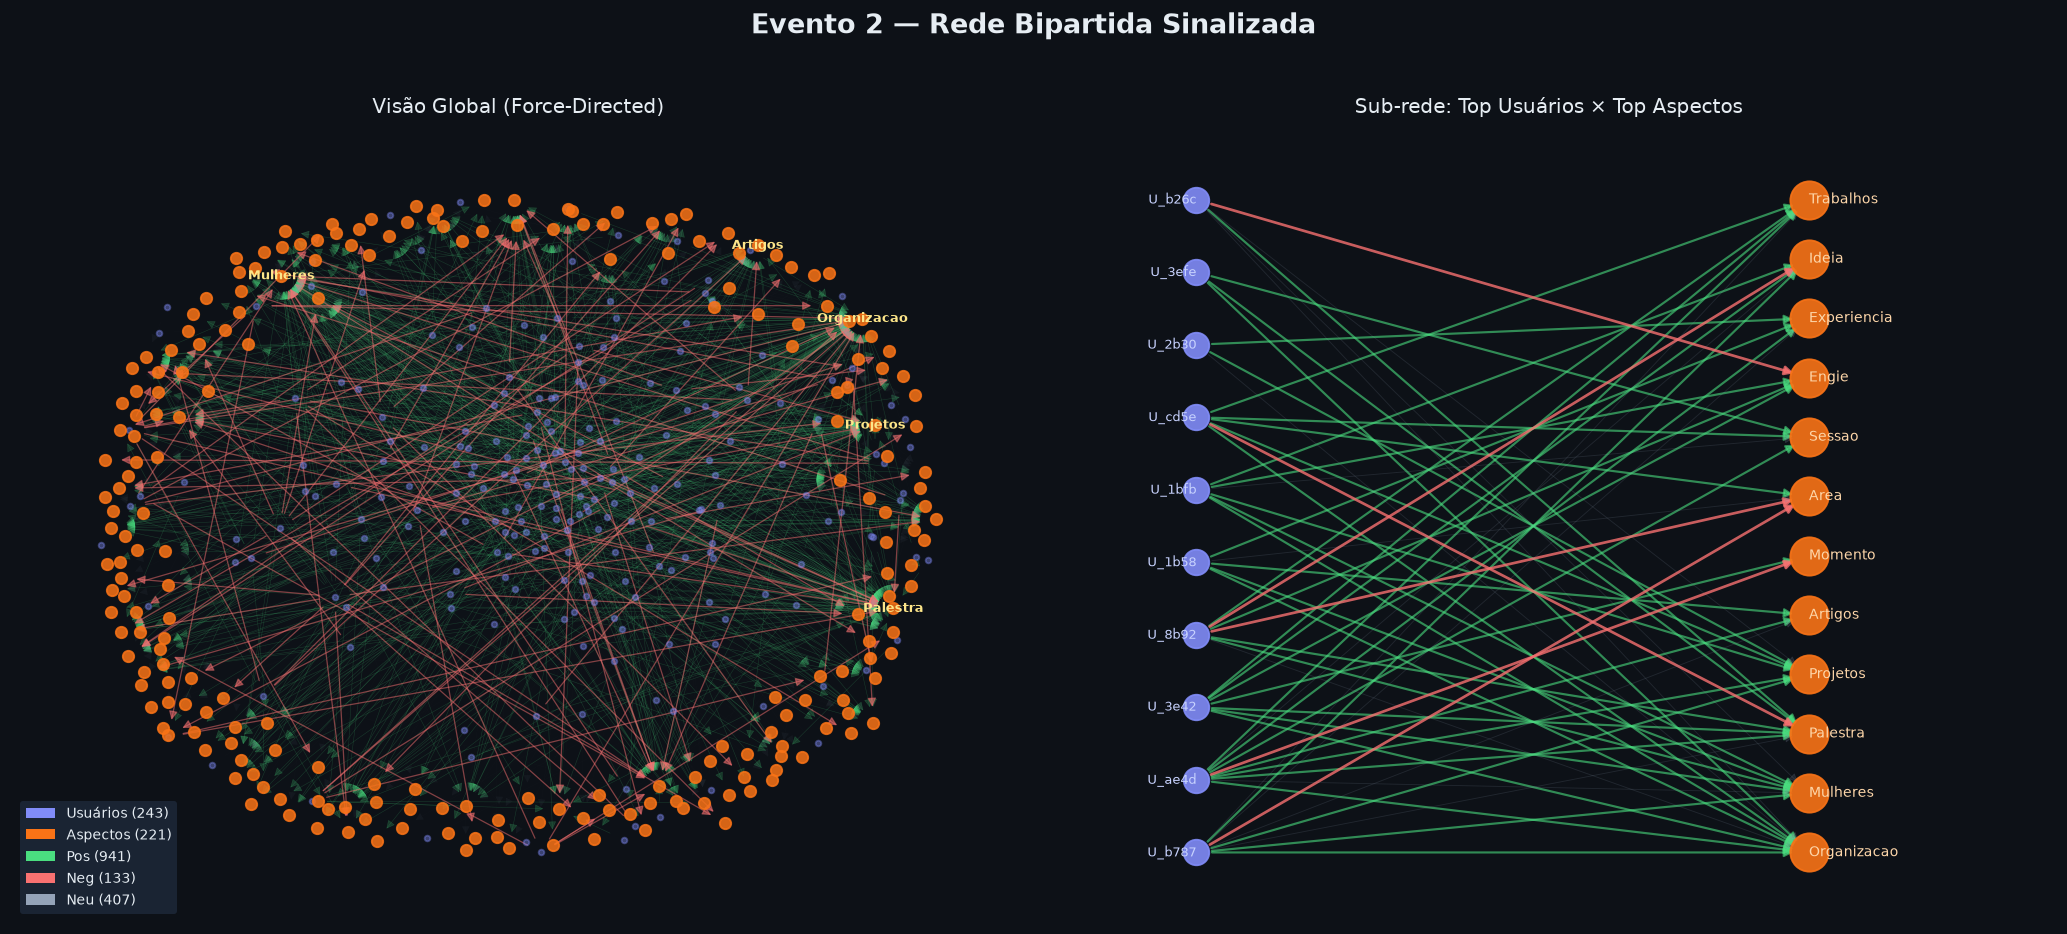
\includegraphics[width=\linewidth]{../resultados/redes/network_comentarios_wit.png}
  \caption{Rede Bipartida Sinalizada - Evento 2 (Engajamento Muito Alto).}
  \label{fig:evt2}
\end{figure}

Este conjunto de dados representa uma dinâmica de fortíssimo engajamento. A rede estrutural foi modelada com 464 nós (sendo 243 usuários e 221 aspectos únicos) e 1.481 arestas sinalizadas (941 positivas, 133 negativas e 407 neutras). A proporção de 0,91 aspectos por usuário demonstra um equilíbrio notável e alto foco avaliativo.

QP1 - Concentração e Polarização: 
A avaliação topológica apontou que os grandes \textit{hubs} de atração estrutural foram Organização (grau = 157), Mulheres (grau = 112) e Palestra (grau = 109). O alto grau de entrada de "Mulheres" revela que as temáticas de gênero formaram a espinha dorsal estrutural do evento. No extremo oposto, problemas como "Preconceito", "Etarismo" e falhas técnicas de "QR Code" apareceram como nós marginais com conectividade baixíssima. Secundariamente, o NSS confirmou a forte aprovação dos hubs e a total rejeição dos nós marginais.

QP2 - Heterogeneidade de Engajamento:
A rede exibe uma distribuição de atividade fortemente heterogênea, aderindo ao padrão \textit{scale-free} (\textit{cauda longa}) clássico descrito por Barabási \cite{barabasi}. Enquanto a minoria dos usuários apresenta baixa atividade (25 emitiram apenas um único comentário), a rede é sustentada por superusuários centrais: 129 participantes emitiram 5 ou mais \textit{feedbacks}, com o topo da cauda registrando incríveis 30 arestas emitidas por uma única pessoa. Estes conectores hiperativos garantiram a conectividade do grafo.

QP3 - Bolhas de Opinião ($G_{user}$):
Ao projetarmos a homofilia de opiniões \cite{easley}, o algoritmo de detecção encontrou 18 comunidades de participantes. As quatro maiores (tamanhos 71, 65, 59 e 34) aglutinam a maior parte dos presentes, demonstrando consenso macro em torno das atividades principais. As comunidades menores representam pequenas bolhas focais, formadas por participantes que discordaram da maioria ou se uniram pela avaliação de aspectos periféricos (ex: grupos isolados discutindo minicursos), provando que a métrica global oculta nichos de experiência.

QP4 - Correlação Estrutural ($G_{entity}$):
A projeção de entidades revelou 48 comunidades temáticas. É fascinante notar que a rede segregou topologicamente as trilhas do evento. A maior comunidade (37 entidades) aglomerou aspectos de administração e infraestrutura, conectando os termos "Agenda", "Apoio" e "Área". Uma comunidade estruturalmente separada e densa (34 entidades) emergiu focada na diversidade, conectando termos como "@mermasdigitais", "Aleteia", "Autoconfiança" e "Animação". Isso comprova matematicamente que as discussões políticas de gênero e as discussões operacionais correram em trilhas de experiência paralelas \cite{blondel}.

QP5 - Intensidade e Sentimento Global:
A intensidade da emoção neste evento foi a maior do \textit{corpus}, atingindo um peso médio de +0,299 por aresta. Como consequência deste forte peso topológico, a métrica comercial (NSS) alcançou a marca de 54,56\%, refletindo a densidade maciça de aprovação.

\subsection{Estudo de Caso: Evento 3 (Engajamento Alto)}

\begin{figure}[H]
  \centering
  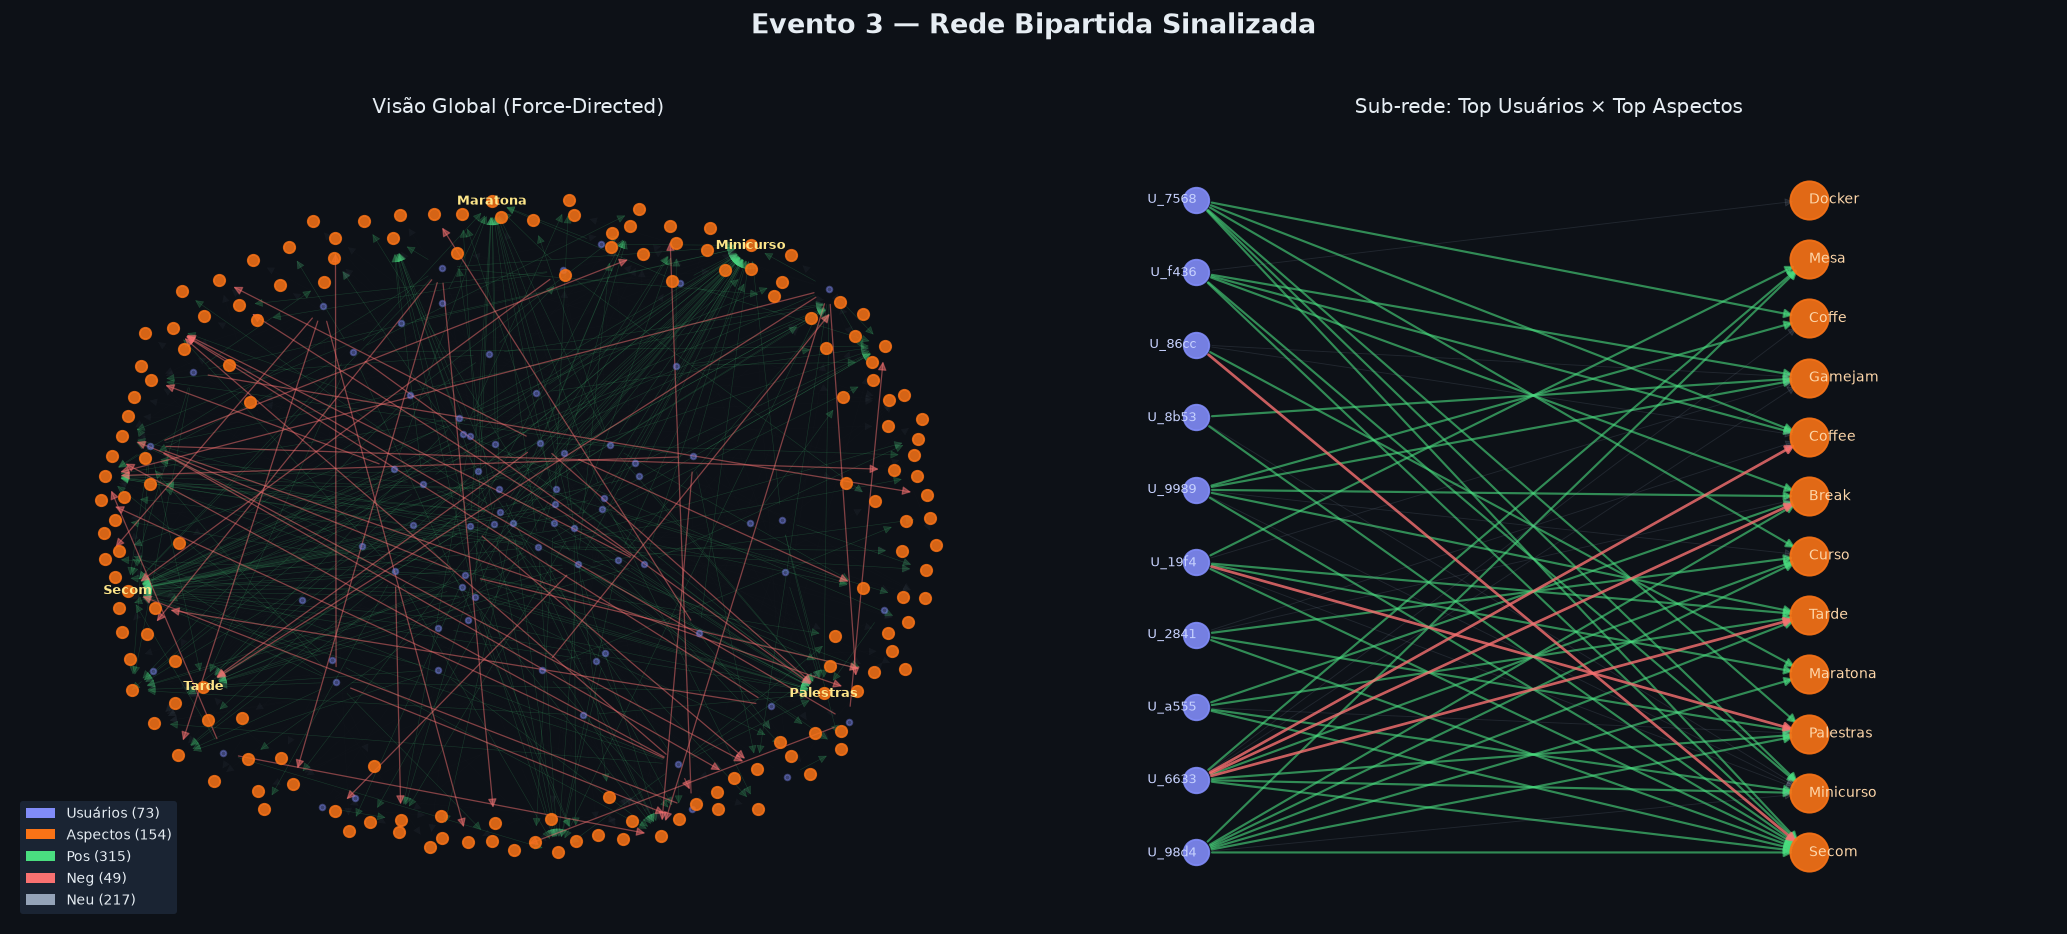
\includegraphics[width=\linewidth]{../resultados/redes/network_secom-xiv.png}
  \caption{Rede Bipartida Sinalizada - Evento 3.}
  \label{fig:evt3}
\end{figure}

Rede com 227 nós (73 usuários, 154 aspectos) e 581 arestas.
QP1: Concentração de arestas em Secom (grau=54) e Minicurso (grau=45). O foco topológico esteve puramente no conteúdo técnico.
QP2: Atividade homogênea e concentrada (média 7,96 por usuário).
QP3 e QP4: Encontraram-se 7 bolhas de opinião de usuários e 57 módulos de entidades, evidenciando grandes blocos de consenso.
QP5: O peso médio da rede registrou +0,208. O altíssimo volume de arestas neutras (37,3\%) indica feedbacks estritamente descritivos. O NSS secundário ficou em 45,78\%.

\subsection{Estudo de Caso: Evento 4 (Engajamento Moderado)}

\begin{figure}[H]
  \centering
  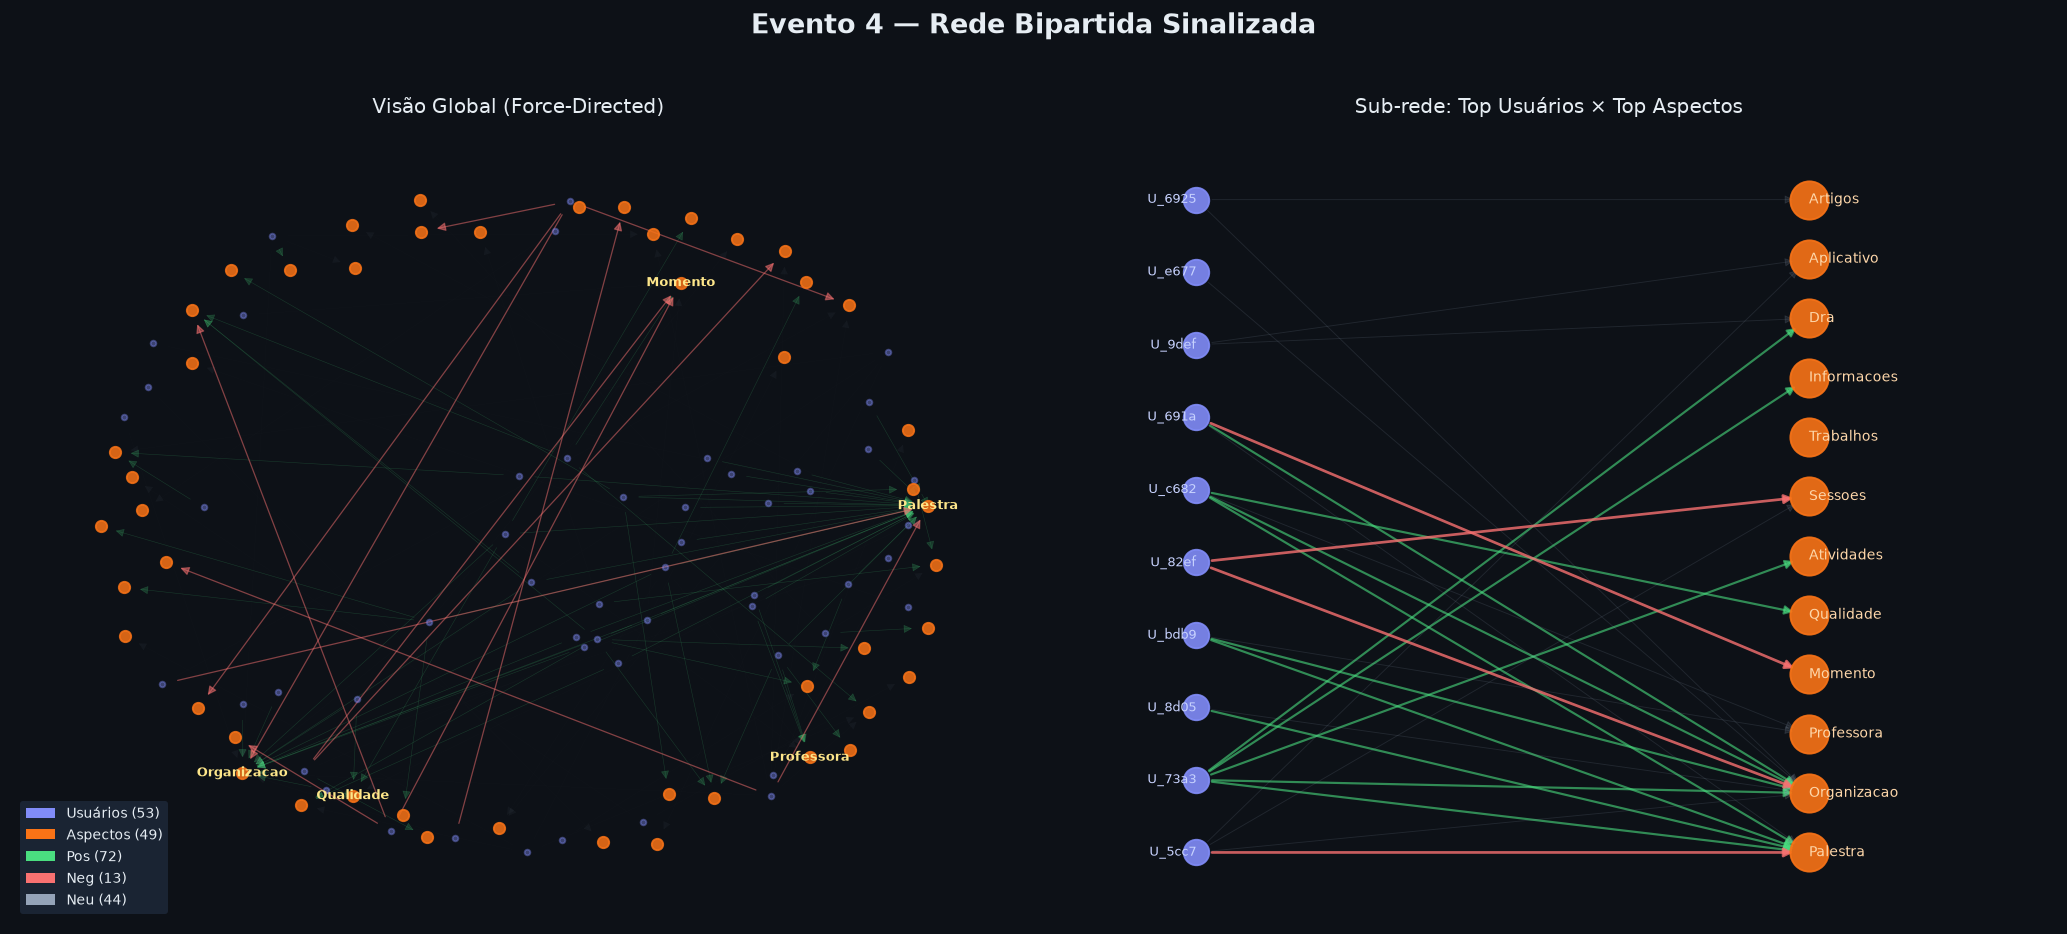
\includegraphics[width=\linewidth]{../resultados/redes/network_sbcas.png}
  \caption{Rede Bipartida Sinalizada - Evento 4.}
  \label{fig:evt4}
\end{figure}

Rede com 102 nós e 129 arestas. 
QP1: Hubs estruturais em Palestra (grau=31) e Organização (grau=20). Destaque fundamental para Professora (grau=5) atuando como uma "ilha topológica de satisfação local" desconexa do resto da percepção \cite{easley}.
QP2 e QP3: Participação casual e fragmentada (grau médio 2,43). A rede não forma componente conexo gigante, gerando 19 micro-comunidades de usuários desarticuladas.
QP4: Apenas 23 comunidades rasas de entidades.
QP5: O Sentimento Médio atingiu +0,279, indicando forte intensidade de aprovação naquelas conexões pontuais. (NSS referencial de 45,74\%).

\subsection{Estudo de Caso: Eventos 5 e 6 (Engajamento Baixo e Micro)}

\begin{figure}[H]
  \centering
  \begin{minipage}{0.48\linewidth}
    \centering
    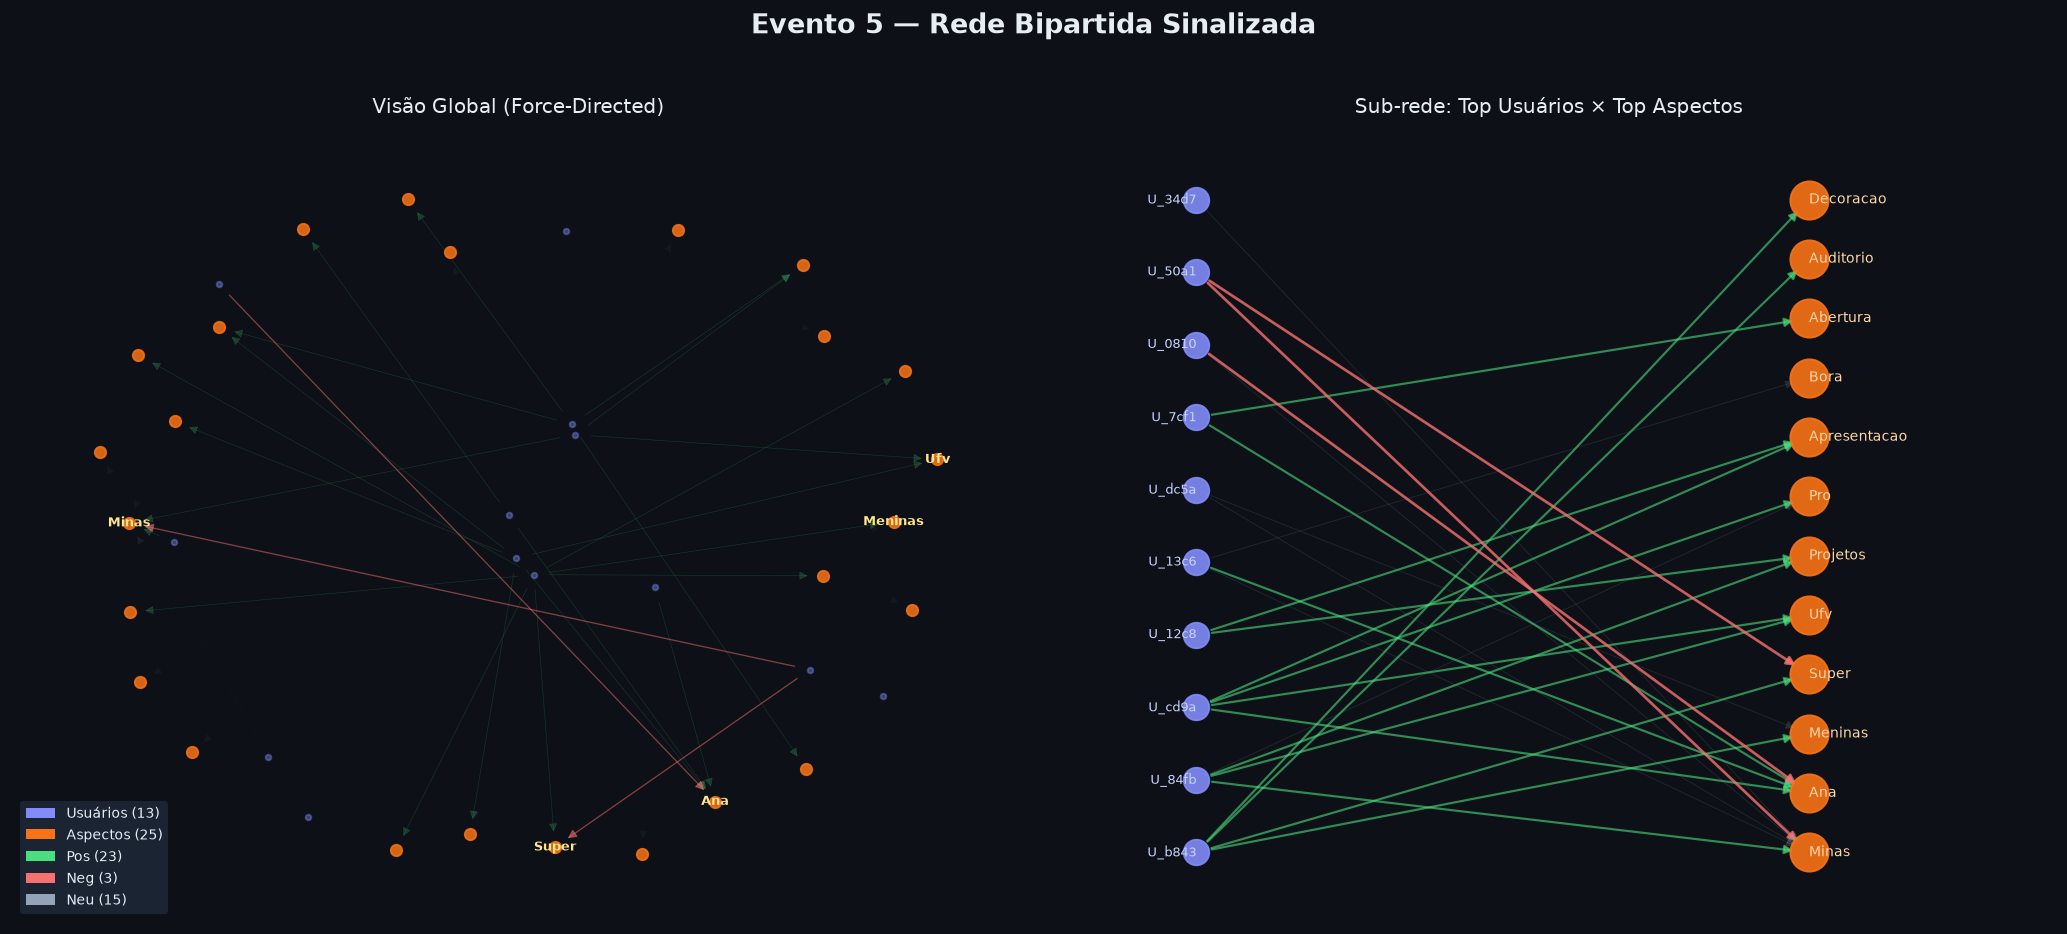
\includegraphics[width=\linewidth]{../resultados/redes/network_minas-coders-day.png}
    \caption{Rede Bipartida - Evento 5.}
    \label{fig:evt5}
  \end{minipage}\hfill
  \begin{minipage}{0.48\linewidth}
    \centering
    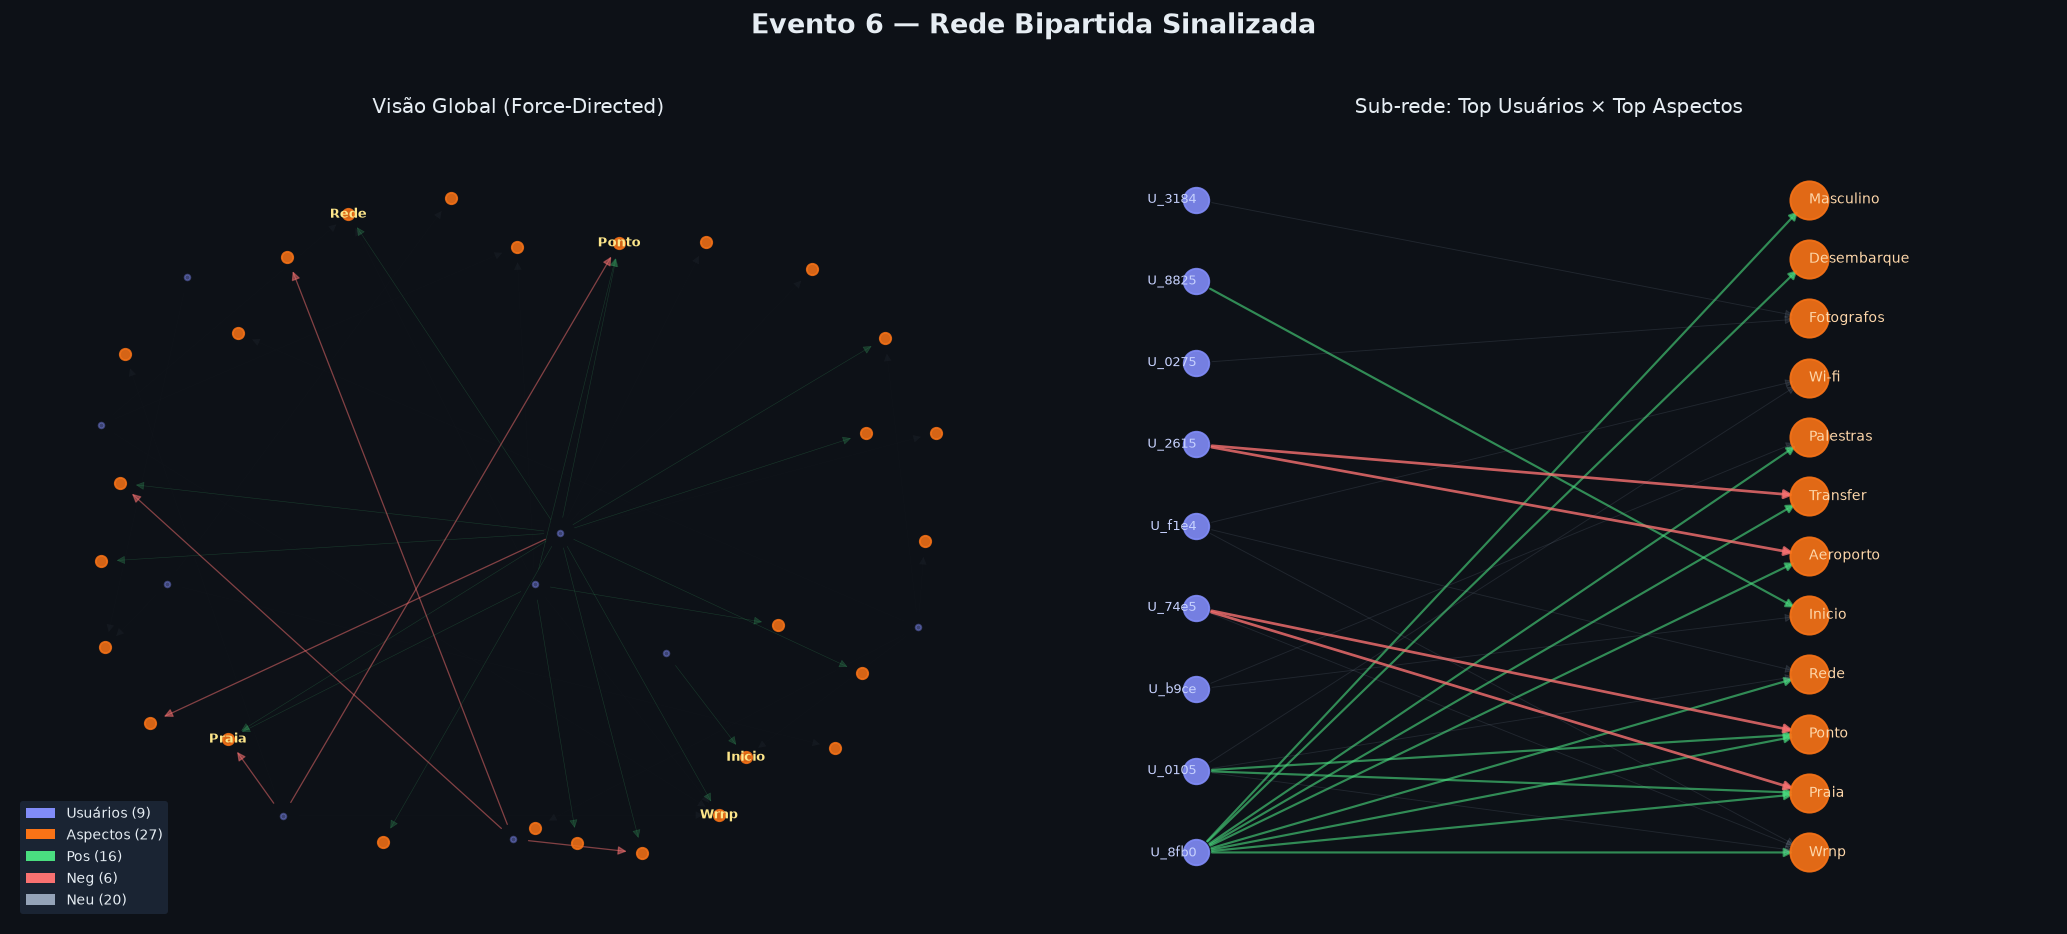
\includegraphics[width=\linewidth]{../resultados/redes/network_wrnp.png}
    \caption{Rede Bipartida - Evento 6.}
    \label{fig:evt6}
  \end{minipage}
\end{figure}

O Evento 5 (38 nós, 41 arestas) e o Evento 6 (36 nós, 42 arestas) geraram redes esparsas. 
Aplicações analíticas de distribuição de cauda longa (QP2) e módulos de Louvain (QP3, QP4) provaram-se não pertinentes para essa escala macro, pois geram apenas agrupamentos isolados triviais. 
No entanto, evidenciou-se a alta suscetibilidade de redes micro a anomalias comportamentais: no Evento 6, um único superusuário isolado gerou 35\% das arestas (15 conexões).

\subsection{Análise de Nós e Subgrafos de Interesse}

Além do mapeamento macro das redes, a modelagem de redes complexas permite focar em nós específicos (aspectos centrais) e extrair os seus subgrafos de vizinhança para compreender o fluxo qualitativo de opiniões, validando teorias clássicas de homofilia e equilíbrio estrutural \cite{easley}.

\subsubsection{Análise do Hub de Diversidade: O Aspecto "Mulheres" (Evento 2)}

O nó representativo do aspecto Mulheres atuou como um dos maiores \textit{hubs} estruturais do Evento 2, registrando um grau de entrada de 112 conexões sinalizadas. Extraiu-se o subgrafo de vizinhança imediata para análise:

\begin{figure}[H]
  \centering
  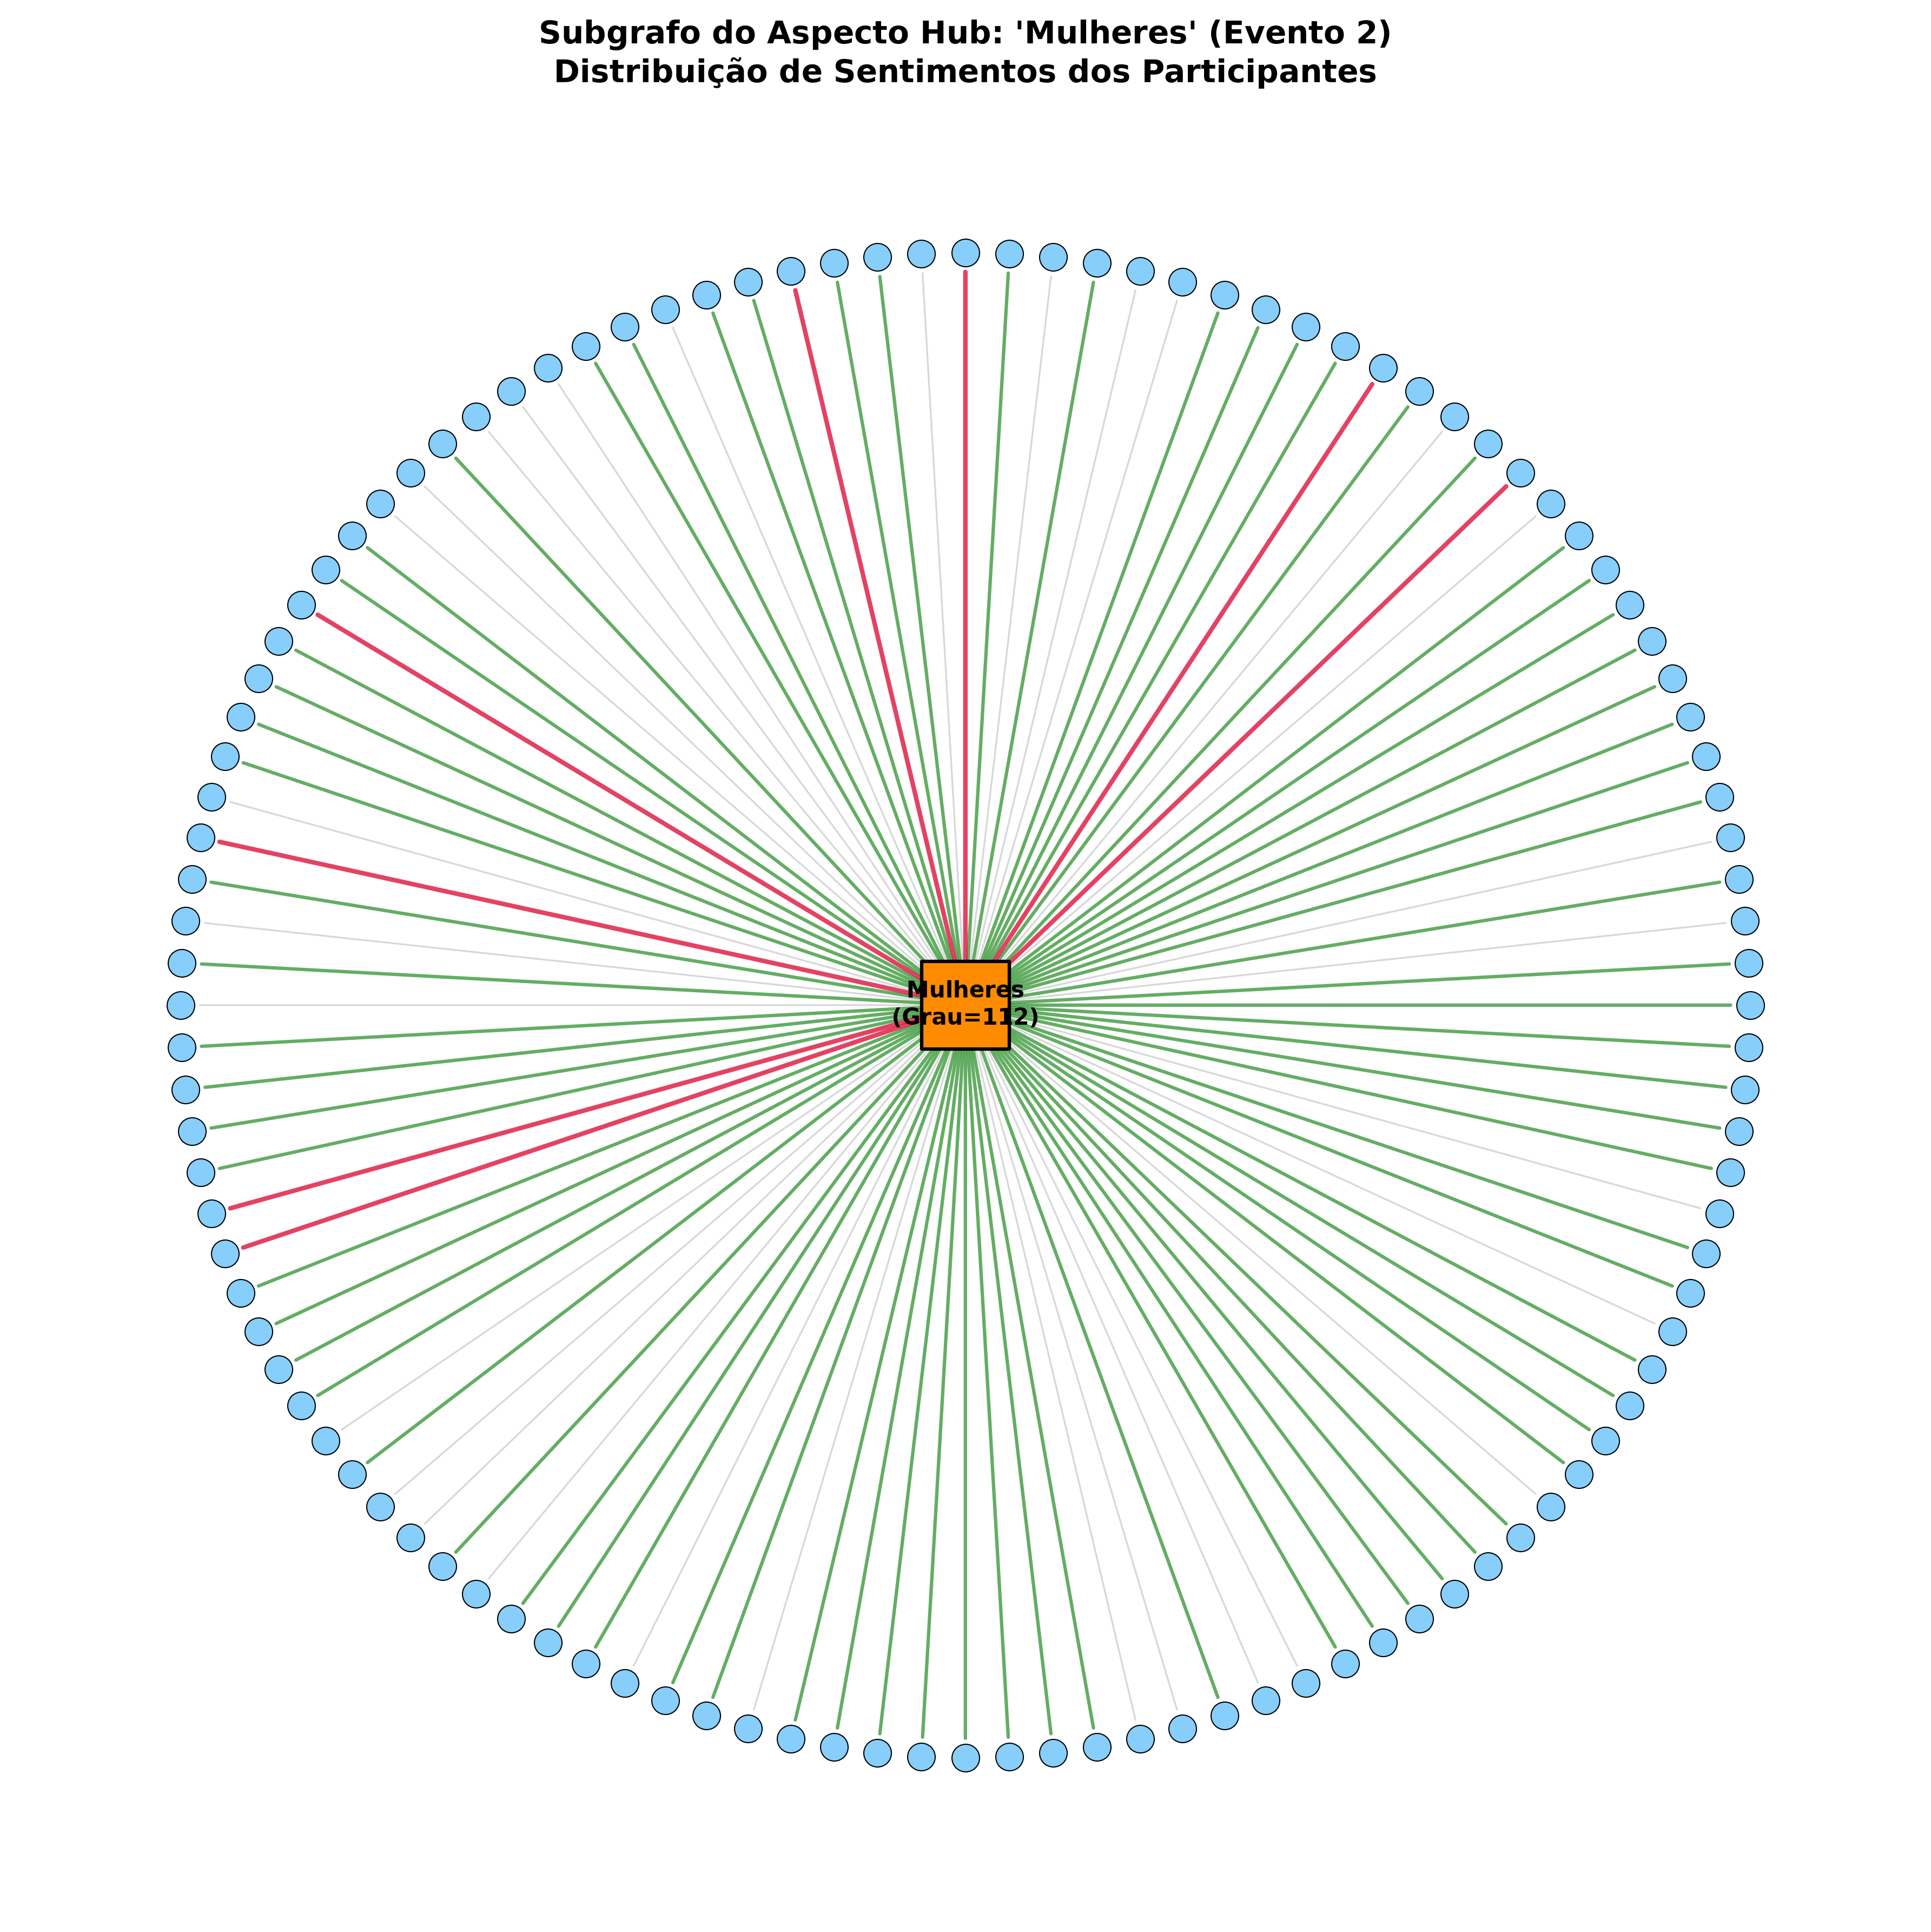
\includegraphics[width=\linewidth]{../resultados/redes/subgrafo_mulheres.png}
  \caption{Subgrafo do Hub "Mulheres" - Evento 2.}
  \label{fig:mulheres}
\end{figure}

A topologia revela uma Estrutura de Estrela (Star Network), onde 112 usuários ocupam a periferia. Mais criticamente, a análise evidencia um Sentimento Predominantemente Coeso e Homofílico: das 112 arestas, 74 são estritamente positivas e apenas 8 são negativas. 

Sob a ótica de Ciência de Redes, este aspecto se consolida como um exemplo de excelência analítica por comprovar:
\begin{enumerate}
    \item Validação Metodológica: O surgimento orgânico do tema central do evento como núcleo de grau elevado valida a assertividade do pipeline NLP (\textit{Aspect-Based Sentiment Analysis}).
    \item Equilíbrio Estrutural: A maciça proporção de conexões positivas demonstra um forte \textit{consenso homofílico} \cite{easley}, onde a estabilidade dos sinais impede a formação de díades de conflito.
    \item Fechamento Focal: O aspecto funciona como o cimento de coesão, conectando estruturalmente participantes de diferentes bolhas isoladas do grafo $G_{user}$.
\end{enumerate}

\subsubsection{Análise do Hub de Sucesso Local: O Aspecto "Professora" (Evento 4)}

No Evento 4, a rede global é altamente esparsa e fragmentada (apenas 53 usuários emitindo uma média de 2,43 comentários esporádicos), incapaz de formar um componente gigante conexo. No entanto, o aspecto Professora desponta organicamente como um formidável \textit{hub} local (grau = 5).

Para analisar o impacto dessa palestrante, extraímos o subgrafo focado neste nó de entidade:

\begin{figure}[H]
  \centering
  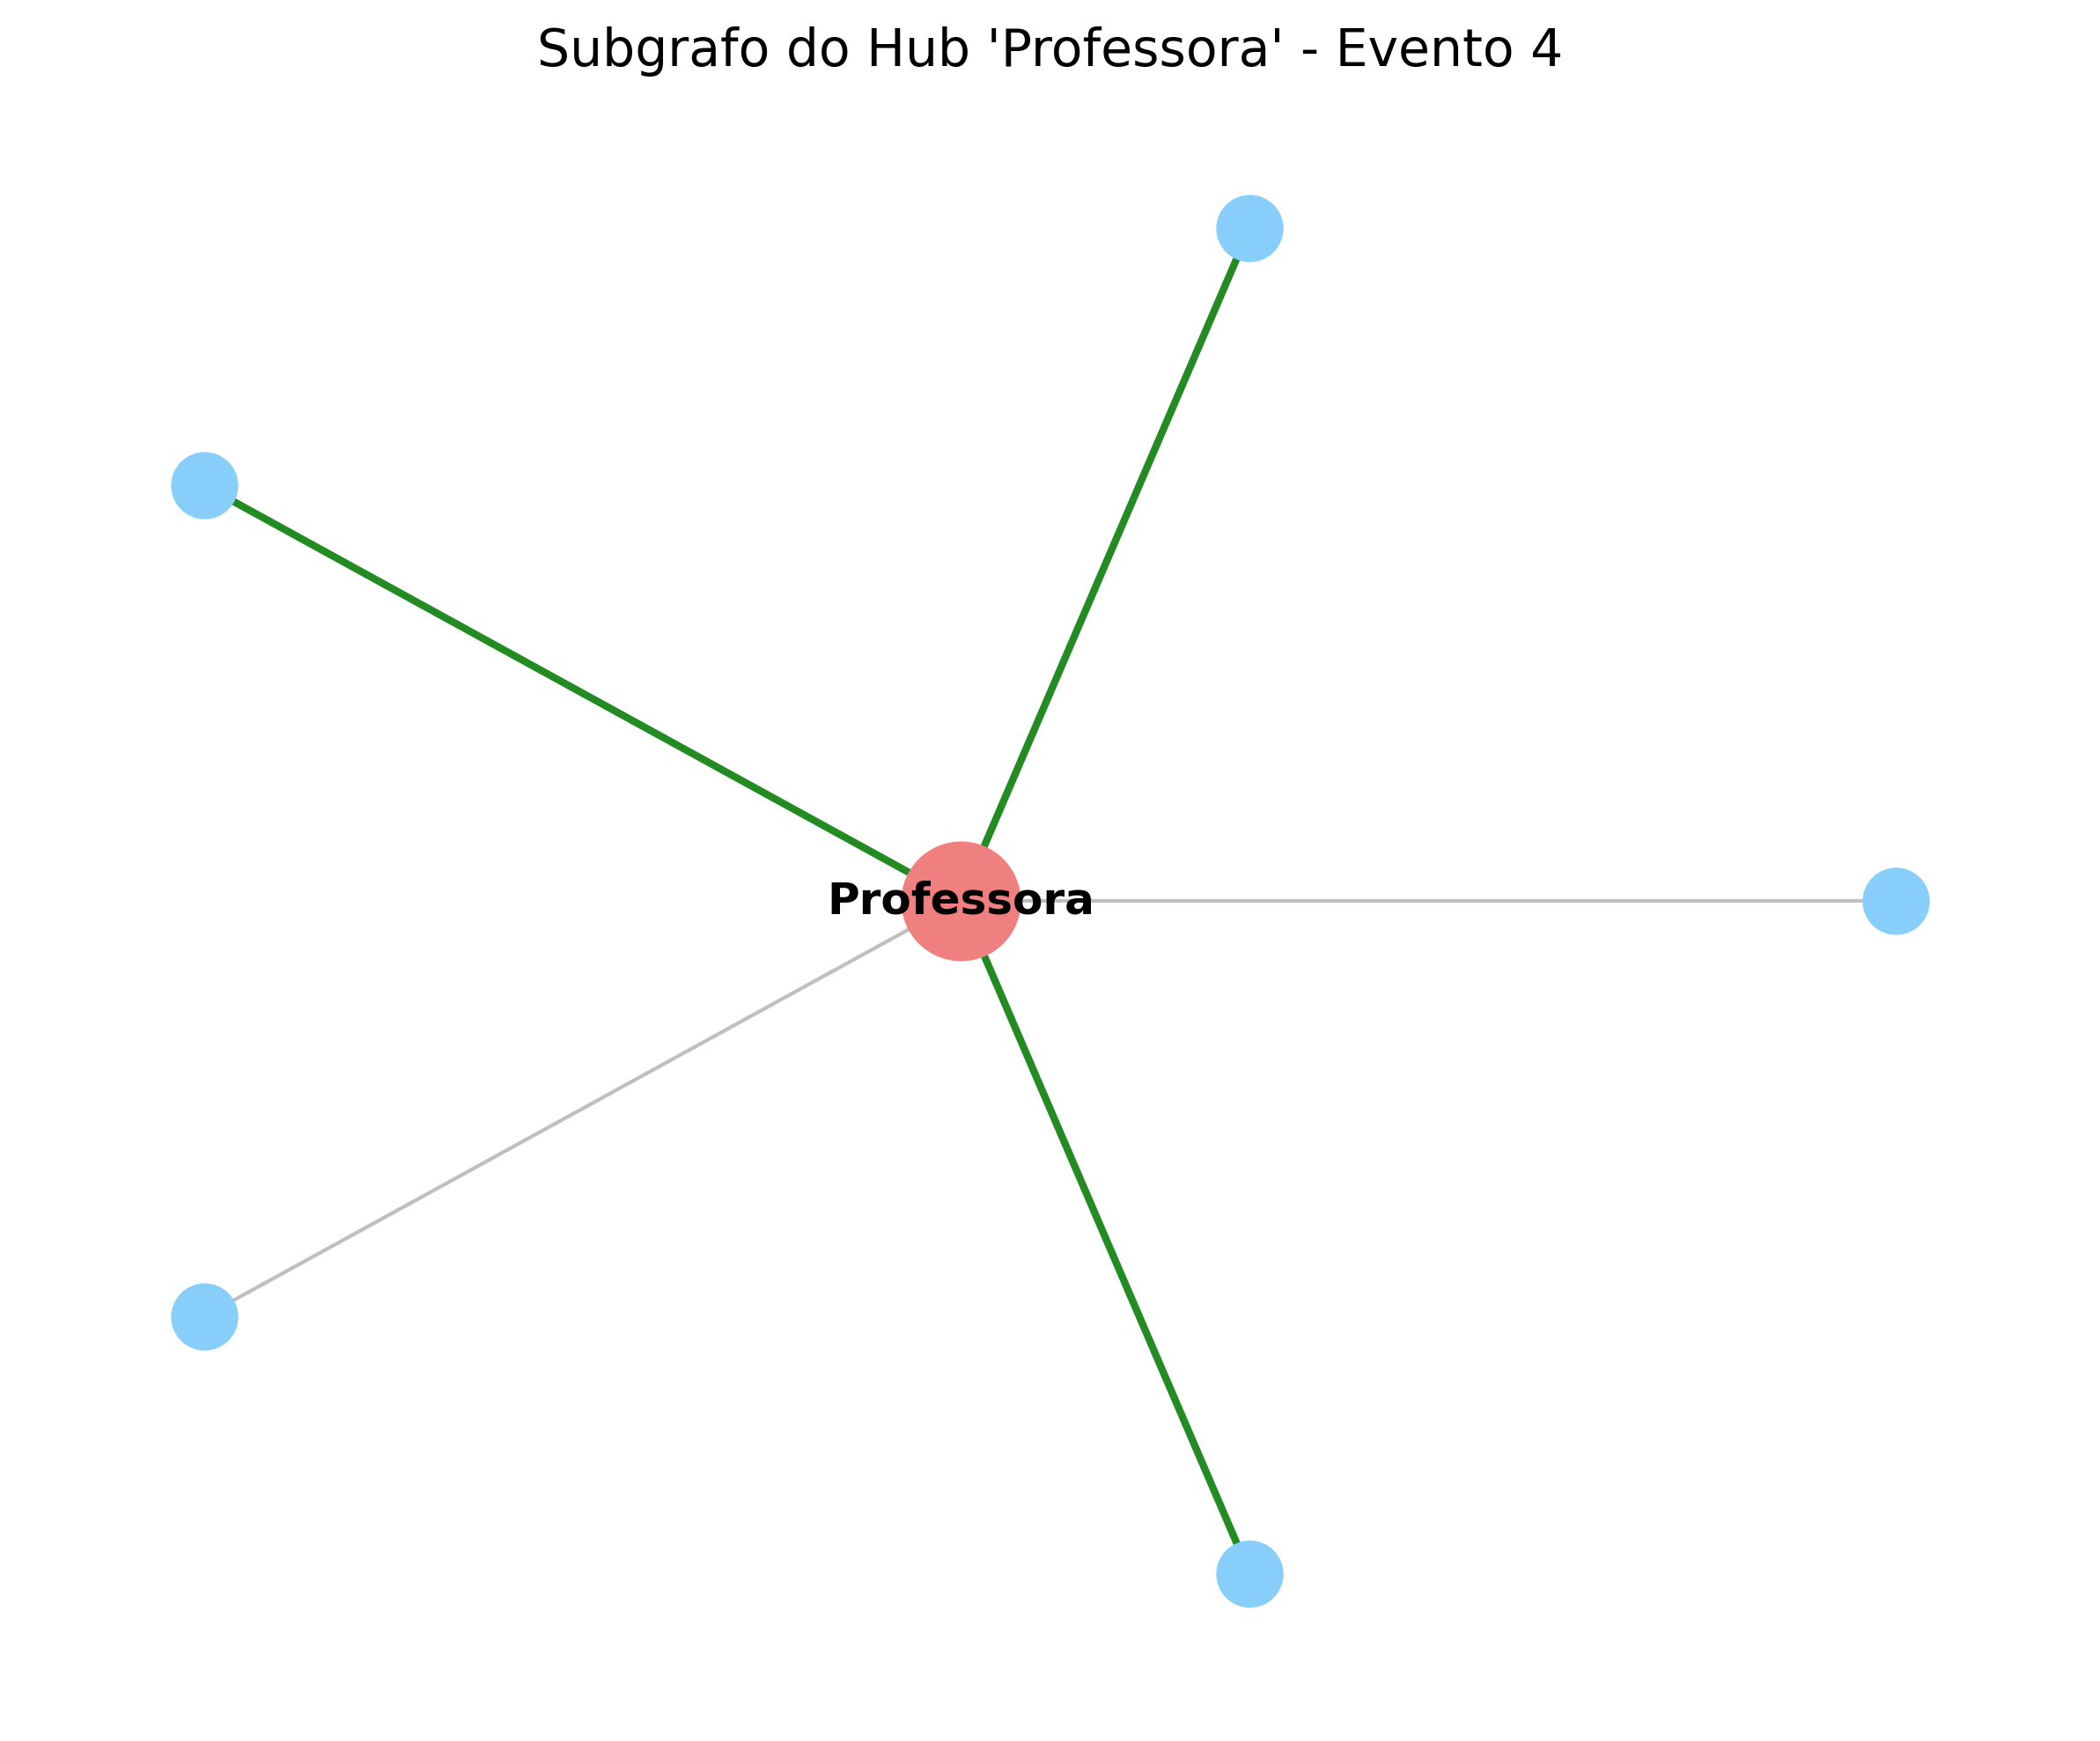
\includegraphics[width=\linewidth]{../resultados/redes/subgrafo_professora.png}
  \caption{Subgrafo do Hub de Sucesso Local "Professora" - Evento 4.}
  \label{fig:professora}
\end{figure}

A topologia deste subgrafo revela as seguintes particularidades estruturais cruciais:
\begin{enumerate}
    \item Consenso Positivo e Ausência de Ruído: A imagem mostra que todas as avaliações recebidas por essa palestrante foram boas ou neutras. Das 5 conexões, 3 são elogios (linhas verdes) e 2 são apenas comentários informativos (linhas cinzas). Não houve nenhuma reclamação (linhas vermelhas).
    \item Ilha de Sucesso Isolada: Como o evento teve baixa participação geral, a rede de conexões ficou bastante vazia e desconectada. Mesmo nesse cenário, o nó da "Professora" conseguiu formar uma "ilha de satisfação" própria \cite{easley}. Para conseguir isso, a palestrante precisou se destacar bastante para motivar essas 5 pessoas a avaliá-la positivamente.
    \item Reconhecimento de Nicho: A extração focal deste subgrafo oferece à gestão do evento uma ferramenta visual clara para identificar e premiar os talentos individuais, garantindo que o sucesso da instrutora seja documentado para futuras edições.
\end{enumerate}

\subsection{Vantagem Topológica: Sentimento Médio vs. Saldo Comercial}

A tabela abaixo sintetiza os resultados estruturais da rede, evidenciando como a topologia pura e o Sentimento Médio (\textit{Score}) fornecem diagnósticos mais profundos que a mera diferença de saldos do NSS:

\begin{table}[H]
\centering
\resizebox{\linewidth}{!}{
\begin{tabular}{lcccccc}
\hline
\textbf{Evento} & \textbf{Usuários} & \textbf{Aspectos} & \textbf{Arestas} & \textbf{Positivo (\%)} & \textbf{Negativo (\%)} & \textbf{Score Médio} \\
\hline
Evento 1 & 112 & 368 & 2.040 & 51,2\% & 13,8\% & +0,179 \\
Evento 2 & 243 & 221 & 1.481 & 63,5\% & 9,0\% & +0,299 \\
Evento 3 & 73 & 154 & 581 & 54,2\% & 8,4\% & +0,208 \\
Evento 4 & 53 & 49 & 129 & 55,8\% & 10,1\% & +0,279 \\
Evento 5 & 13 & 25 & 41 & 56,1\% & 7,3\% & +0,243 \\
Evento 6 & 9 & 27 & 42 & 38,1\% & 14,3\% & +0,161 \\
\hline
\end{tabular}
}
\caption{Comparativo Geral Estrutural dos Eventos Analisados.}
\label{tab:comparativo}
\end{table}

Comparar as redes com as notas comerciais (como o NSS) mostra o maior problema de usar médias simples: achar que todo o público pensa igual. O NSS apenas subtrai a porcentagem de críticas da porcentagem de elogios para gerar uma nota única. O perigo disso é que uma nota final neutra ou "zero" não significa que todos acharam o evento razoável. Na verdade, o público pode estar totalmente dividido em dois grupos extremos (metade adorou muito e metade odiou muito) \cite{easley}. Ao construir a rede de interações, conseguimos ver claramente a formação dessas "bolhas" de opinião e entender o que agradou cada grupo, em vez de sermos enganados por uma nota geral cega.

Além de mostrar como o público se divide, a análise em rede protege a organização contra usuários problemáticos ou exagerados. Em sistemas que só contam o volume de mensagens, uma única pessoa que envia dezenas de críticas seguidas (como aconteceu no Evento 6) acaba derrubando a nota do evento inteiro sozinha. Isso faz a organização pensar que o evento foi um fracasso geral. Já na rede estruturada, esse usuário exagerado é facilmente descoberto: ele aparece no gráfico como um ponto extremamente agitado, mas isolado da maioria das pessoas. Isso permite que a gestão ignore esse "ruído" e foque na opinião real da maioria da rede.

Por fim, usar o peso matemático das conexões na rede (Sentimento Médio) se mostrou muito mais preciso. Enquanto as porcentagens e notas globais escondem os pequenos sucessos (como a ótima avaliação que a "Professora" recebeu no Evento 4) só porque o evento inteiro teve pouca participação, a análise de rede permite extrair apenas as conexões daquela pessoa. Isso garante que talentos individuais sejam reconhecidos e elogiados de forma justa, sem que a nota baixa do resto do evento atrapalhe a avaliação deles.

\section{Considerações Éticas}
Em projetos que analisam redes de interações humanas, proteger a identidade dos participantes é essencial. Por isso, todos os feedbacks recolhidos na plataforma foram anonimizados, substituindo os nomes reais por códigos de identificação (UUIDs). Isso garantiu que os usuários pudessem expressar suas opiniões, inclusive críticas e reclamações, totalmente livres de qualquer risco de exposição. Além disso, ao utilizarmos simulações de dados e processamento de linguagem, tomamos o cuidado de calibrar os algoritmos para que eles não eliminassem opiniões divergentes ou criassem uma rede artificialmente otimista, mantendo o retrato real e transparente de cada evento.

\section{Conclusão}
Este projeto demonstrou na prática o potencial de integrar a modelagem de Redes Complexas à avaliação de eventos. A projeção de grafos bipartidos revelou dinâmicas valiosas, como a formação de bolhas de opinião, o impacto estrutural de superusuários e o sucesso isolado de serviços específicos. Mapear essas interações entrega aos organizadores uma ferramenta diagnóstica profunda, permitindo que a gestão tome decisões estratégicas baseadas na estrutura real de experiência do público.

\bibliographystyle{ACM-Reference-Format}
\bibliography{sample-base}

\end{document}
